\documentclass[10pt,journal,compsoc]{IEEEtran}

\usepackage{amsmath,amssymb,amsfonts}
\usepackage{algorithmic}
\usepackage{graphicx}
\usepackage{textcomp}
\usepackage{xcolor}
\usepackage{booktabs}
\usepackage{multirow}
\usepackage{array}
\usepackage{url}
\usepackage{cite}
\usepackage{subcaption}
\usepackage{hyperref}
\usepackage{siunitx}

\hypersetup{
    colorlinks=true,
    linkcolor=blue,
    citecolor=blue,
    urlcolor=blue
}

\begin{document}

\title{Plane-Aware Joint Learning for Brain Tumor Classification and Delineation:\\ Multi-Task Benchmarking, Explainability, and External Generalization Under Domain Shift}

\author{Tareque~Mohammad,~and~Collaborators%
\thanks{Manuscript received September 8, 2026. This research was supported by the Advanced Biomedical Imaging and Computing Laboratory. (Corresponding author: Tareque Mohammad).}%
\thanks{The authors are with the Department of Computer Science and Biomedical Engineering.}}

\markboth{IEEE Transactions on Medical Imaging,~Vol.~XX, No.~X, September~2026}%
{Mohammad \MakeLowercase{\textit{et al.}}: Plane-Aware Joint Learning for Brain Tumor Analysis}

\IEEEtitleabstractindextext{%
\begin{abstract}
Accurate computational analysis of intracranial neoplasms from magnetic resonance imaging (MRI) demands both reliable histologic classification and precise spatial delineation of tumor margins. Most contemporary architectures treat these as decoupled pipelines and ignore the anatomical acquisition plane (axial, sagittal, coronal) in which each slice was acquired. We propose PAUMT-Net, a unified plane-aware joint learning architecture that processes individual 2D MRI slices via a shared ResNet34 backbone, a learned plane embedding, a two-layer classification head, and a UNet decoder modulated by Feature-wise Linear Modulation (FiLM). A plane-marginalized inference strategy enables zero-shot external deployment without plane annotations. We identify and correct a critical training-pipeline bug wherein healthy scans lacking mask files were silently excluded from segmentation supervision, causing a 95.71\% false-positive rate (reduced to 0.00\% post-correction). On the held-out BRISC2025 test set (1,000 slices), PAUMT-Net achieves 99.30\%\,$\pm$\,0.10\% classification accuracy (95\% CI: [98.70\%, 99.80\%]), 99.38\%\,$\pm$\,0.11\% macro F1, and 87.93\%\,$\pm$\,0.26\% segmentation Dice across three independent seeds. Paired Wilcoxon testing confirms statistically significant segmentation improvement from plane conditioning ($p = 0.0344$). Zero-shot evaluation on the PMRAM dataset (N=1,410) achieves 92.41\% accuracy, while AJBDS-2023 (N=4,826 slices) reveals severe segmentation domain degradation (38.35\% tumor Dice, 36.31\% empty-slice hallucination rate) mitigated via test-time threshold calibration ($\tau = 0.85$). These findings establish that joint multi-task learning provides foundational regularization while plane conditioning refines spatial boundaries, and highlight the pronounced vulnerability of dense segmentation to domain shift compared to classification.
\end{abstract}

\begin{IEEEkeywords}
Brain tumor, MRI classification, tumor boundary delineation, multi-task learning, anatomical-plane conditioning, Grad-CAM explainability, model calibration, domain shift, external validation, BRISC2025.
\end{IEEEkeywords}}

\maketitle
\IEEEdisplaynontitleabstractindextext
\IEEEpeerreviewmaketitle

\section{Introduction}
\IEEEPARstart{P}{rimary} and metastatic intracranial neoplasms represent a severe healthcare burden globally. Magnetic resonance imaging (MRI) serves as the definitive non-invasive modality for neuro-oncological evaluation, facilitating tumor type differentiation, surgical margin delineation, mass-effect assessment, and longitudinal therapeutic monitoring. In routine diagnostic workflows, neuro-radiologists simultaneously determine tumor histopathology (e.g., distinguishing gliomas, meningiomas, and pituitary adenomas) and map structural lesion margins. In contrast, deep learning literature overwhelmingly bifurcates these tasks into isolated classification networks \cite{he2016deep, fateh2026brisc, tas2026attention, ahmed2026enhancing} or independent segmentation pipelines \cite{ronneberger2015u, fateh2025swinhafnet, alkharaan2026brain}.

Multi-task learning (MTL) offers an appealing paradigm to unify these complementary objectives \cite{caruana1997multitask}. By optimizing a shared visual backbone across classification and segmentation targets, MTL provides an inductive bias that regularizes feature representations and mitigates overfitting to spurious non-pathological imaging shortcuts \cite{zhang2018overview, chen2025cooperative}. Nevertheless, naive multi-task formulations often trigger optimization conflicts and negative gradient interference when tasks exhibit divergent loss landscapes and convergence velocities \cite{sener2018multi, kendall2018multi}.

A second fundamental, yet consistently neglected, dimension in 2D brain MRI analysis is anatomical slice acquisition orientation. Clinical brain protocols routinely acquire images across three mutually orthogonal planes:
\begin{enumerate}
    \item \textbf{Axial (transverse)}: Traverses superior to inferior, delineating hemispheric symmetry and ventricular boundaries.
    \item \textbf{Sagittal}: Traverses lateral to medial, capturing the midline craniocervical junction, brainstem, and sellar compartment.
    \item \textbf{Coronal}: Traverses anterior to posterior, visualizing temporal lobe anatomy, skull base structures, and cranial nerve trajectories.
\end{enumerate}

Intracranial neoplasm morphology diverges drastically across these acquisition views. For instance, a pituitary adenoma in the sagittal orientation presents neatly confined within the sella turcica, whereas its coronal projection highlights suprasellar extension and optic chiasm compression. Conventional deep architectures operate in a plane-agnostic fashion, forcing the encoder to absorb orientation-driven appearance variance implicitly. Explicit conditioning on slice acquisition plane enables neural networks to allocate representational capacity selectively and adapt spatial filters dynamically \cite{stelzner2024recognition, perez2018film}.

A naive inclination in multi-plane MRI datasets is to aggregate slices into multi-view triplets (axial, sagittal, coronal) under the assumption of synchronized patient anatomy. However, a forensic investigation into the benchmark BRISC2025 dataset \cite{fateh2026brisc} reveals that patient-level identifiers are absent; numeric file tokens represent sequential dataset counters rather than subject IDs. Enforcing artificial multi-view groupings across non-identical patient scans introduces fabricated anatomical correspondences devoid of clinical validity.

To resolve these challenges rigorously, we propose the \textbf{Plane-Aware Single-Image Joint Learning Framework (PAUMT-Net)}. Each slice is processed independently, with its anatomical acquisition plane supplied as categorical metadata that modulates the shared encoder and UNet decoder via learned embeddings and Feature-wise Linear Modulation (FiLM) \cite{perez2018film}. The overall architecture is illustrated in Fig.~\ref{fig:architecture}.

\begin{figure*}[t]
\centering
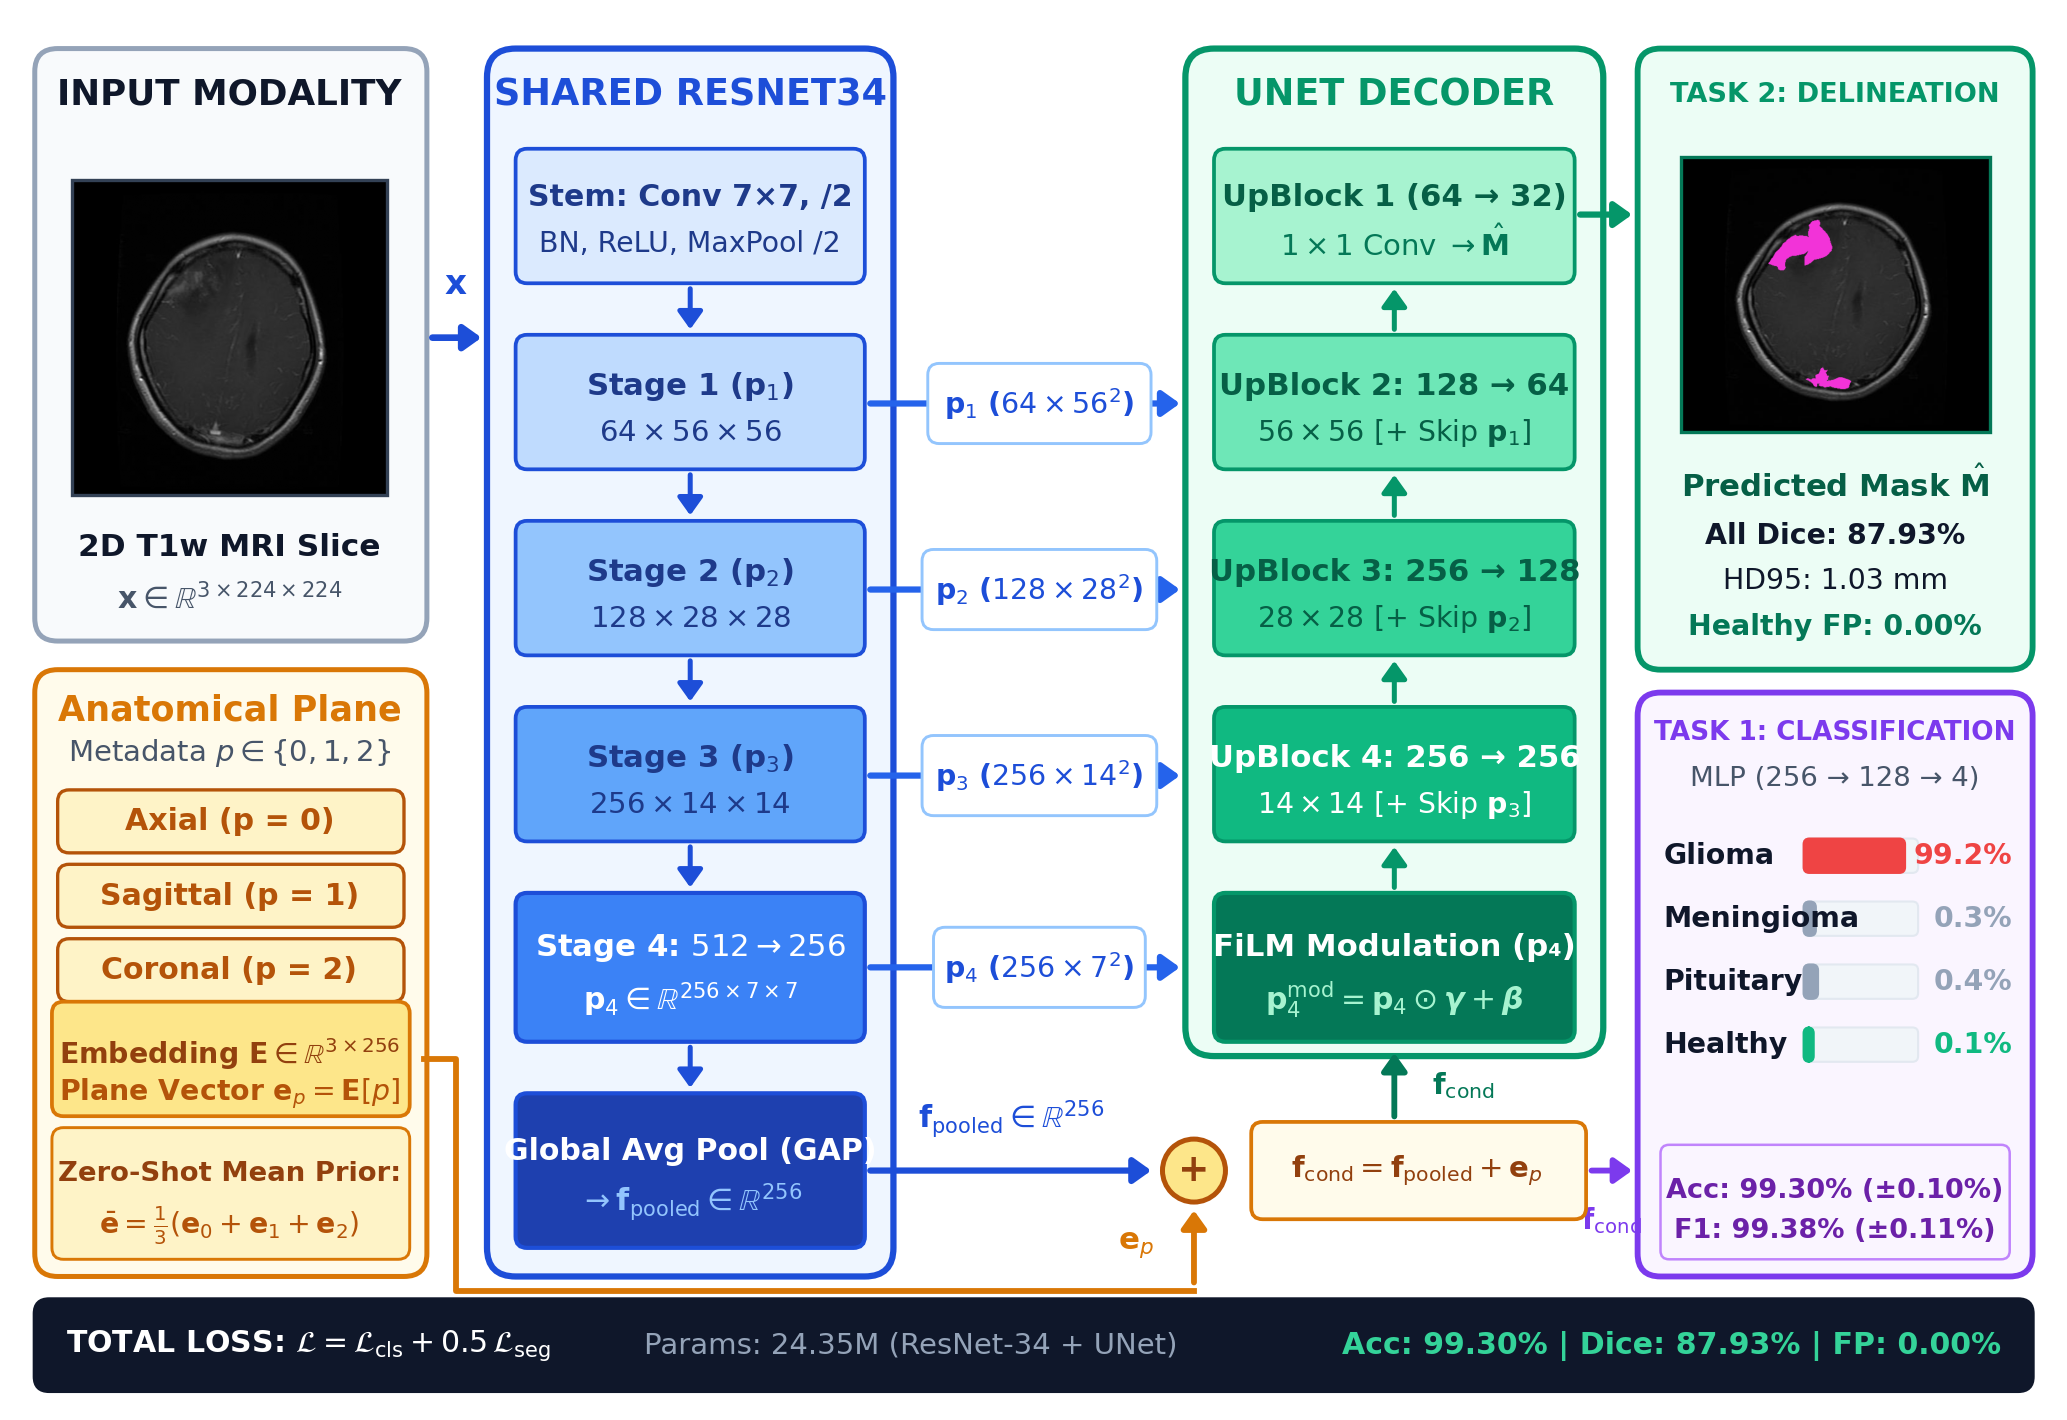
\includegraphics[width=\textwidth]{../figures/journal/figure1_architecture.png}
\caption{PAUMT-Net architecture overview. Input 2D MRI slices ($3 \times 224 \times 224$) are processed by a shared ResNet34 backbone producing hierarchical feature maps $\{\mathbf{p}_1, \ldots, \mathbf{p}_4\}$. A learned plane embedding $\mathbf{e}_p$ is added to the globally pooled bottleneck representation $\mathbf{f}_{\text{pooled}}$, yielding the plane-conditioned vector $\mathbf{f}_{\text{cond}}$. This conditions (a) a two-layer MLP classification head producing class logits $\hat{\mathbf{y}}$ and (b) a UNet decoder via FiLM modulation at the deepest skip connection, producing the segmentation logit map $\hat{\mathbf{M}}$. At external deployment without plane labels, $\mathbf{e}_p$ is replaced by the mean-plane prior $\bar{\mathbf{e}}$.}
\label{fig:architecture}
\end{figure*}

The core contributions of this study are:
\begin{enumerate}
    \item \textbf{Unified Plane-Aware Multi-Task Framework}: We introduce a lightweight, end-to-end multi-task architecture (24.35M parameters) that concurrently classifies brain tumor categories and segments lesion margins, conditioning latent representations on anatomical plane metadata without unsupported patient-grouping assumptions.
    \item \textbf{Supervision Integrity Discovery and Resolution}: We expose and resolve a training-pipeline omission wherein healthy scans lacking mask files were silently excluded from segmentation loss computation, producing a catastrophic 95.71\% false-positive rate on healthy tissue prior to correction (0.00\% post-correction).
    \item \textbf{Rigorous Statistical and Calibration Auditing}: Through 1,000-sample bootstrap resampling, paired McNemar's tests, and Wilcoxon signed-rank tests, we demonstrate that plane conditioning delivers statistically significant segmentation gains on tumor-containing slices ($p = 0.0344$), establishing that joint learning anchors representation stability while plane conditioning refines spatial boundary delineation.
    \item \textbf{Visual Saliency and Explainability}: We extract Grad-CAM heatmaps across all four diagnostic classes and all three acquisition planes, verifying that shared encoder representations focus on intra-axial and extra-axial neoplastic pathology rather than skull contours or background noise.
    \item \textbf{Plane-Marginalized External Generalization \& Domain Shift Diagnostics}: We devise a plane-marginalized inference mechanism ($\mathbb{E}_p[e_p]$) enabling zero-shot external evaluation on PMRAM (N=1,410) and AJBDS-2023 (N=4,826 paired slices). We quantify the pronounced domain gap—where global classification transfers robustly ($>$92\%) while dense segmentation suffers severe degradation—and establish test-time threshold calibration ($\tau = 0.85$) as an actionable mitigation strategy.
\end{enumerate}

\section{Related Work and Benchmark Landscape}
\subsection{Brain Tumor Classification}
Convolutional and Transformer-based models have established strong benchmark results on curated brain MRI datasets \cite{cheng2015enhanced, menze2014multimodal, fateh2026brisc}. Fateh \textit{et al.} \cite{fateh2026brisc} introduced the BRISC2025 benchmark, evaluating ResNet50, EfficientNet-B0, and MobileViT as isolated classification baselines. Subsequent studies explored attention mechanisms \cite{tas2026attention}, artificial colormap transformations with Vision Transformers \cite{ahmed2026enhancing}, and cascaded dual-model pipelines \cite{alkharaan2026brain, linija2026transformer, srinivas2026dual}. However, these approaches address classification in isolation, omitting spatial tumor localization.

\subsection{Brain Tumor Segmentation}
UNet \cite{ronneberger2015u} and its variants remain foundational in medical image segmentation. On BRISC2025, Fateh \textit{et al.} \cite{fateh2025swinhafnet} introduced Swin-HAFNet, integrating Swin Transformer blocks with a hybrid attention decoder. While achieving high Dice scores, Swin-HAFNet operates exclusively on boundary delineation, discarding multi-class diagnostic context. Three-dimensional volumetric methods such as VoxResNet \cite{chen2018voxresnet} and multi-modal BraTS-based segmentation \cite{menze2014multimodal} remain dominant in fully volumetric settings, but require 3D data unavailable in 2D slice-level benchmarks such as BRISC2025.

\subsection{Joint Multi-Task Architectures}
Multi-task architectures combining classification and segmentation have shown efficacy in general medical imaging \cite{zhang2018overview, caruana1997multitask, chen2025cooperative, rui2025automatic, nazir2024end}. Chen \textit{et al.} \cite{chen2025cooperative} demonstrated cooperative multi-task learning for glioma molecular subtyping. Rui \textit{et al.} \cite{rui2025automatic} unified pituitary adenoma segmentation and cavernous sinus invasion. However, existing frameworks rarely account for anatomical slice acquisition geometry or evaluate zero-shot cross-hospital generalization under domain shift.

\subsection{Plane-Aware Conditioning}
Conditioning neural networks on acquisition-plane metadata has been explored for lumbar spine MRI segmentation \cite{stelzner2024recognition} and sMRI-based disease classification using plane-aware Mixture-of-Experts routing \cite{kumar2026pam}. The general framework of Feature-wise Linear Modulation (FiLM) \cite{perez2018film} provides a principled mechanism for injecting categorical conditioning information into convolutional feature maps. To our knowledge, no prior work applies plane-aware FiLM conditioning to joint classification and segmentation on brain tumor 2D slice benchmarks.

\subsection{Domain Generalization in Medical Imaging}
Cross-domain generalization represents a fundamental challenge in clinical AI deployment, where source and target distributions diverge due to scanner heterogeneity, imaging protocol variance, and institutional processing pipelines \cite{dawood2023uncertainty}. Test-time adaptation methods \cite{luo2021semi} and decision-threshold calibration are practical strategies for mitigating domain-induced performance degradation without requiring target-domain retraining.

\subsection{State-of-the-Art Benchmark Comparison}
Table~\ref{tab:sota_comparison} details a comprehensive audit of published 2024--2026 models on the BRISC2025 benchmark.

\begin{table*}[t]
\caption{State-of-the-Art Benchmark Comparison on the BRISC2025 Dataset}
\label{tab:sota_comparison}
\centering
\small
\resizebox{\textwidth}{!}{%
\begin{tabular}{llccccc}
\toprule
\textbf{Method} & \textbf{Architecture} & \textbf{Task Formulation} & \textbf{Parameters} & \textbf{Cls Acc (\%)} & \textbf{Seg Dice (\%)} & \textbf{Healthy FP (\%)} \\
\midrule
Fateh \textit{et al.} (2026) \cite{fateh2026brisc} & ResNet50 & Classification-only & 25.6M & 98.60\% & --- & --- \\
Fateh \textit{et al.} (2026) \cite{fateh2026brisc} & EfficientNet-B0 & Classification-only & 5.3M & 98.20\% & --- & --- \\
Fateh \textit{et al.} (2026) \cite{fateh2026brisc} & Standard UNet & Segmentation-only & 31.0M & --- & 82.40\% & Not reported \\
Swin-HAFNet (2025) \cite{fateh2025swinhafnet} & Swin + Hybrid Attn & Segmentation-only & $\sim$38.0M & --- & 86.50\% & Not reported \\
Ta{\c{s}} \& {\"O}ztepe (2026) \cite{tas2026attention} & Attn-CNN & Classification-only & $\sim$28.0M & 98.90\% & --- & --- \\
Ahmed (2026) \cite{ahmed2026enhancing} & Colormap + ViT-B/16 & Classification-only & 86.6M & 99.10\% & --- & --- \\
Alkharaan \textit{et al.} (2026) \cite{alkharaan2026brain} & EfficientNet + UNet++ & Two-Stage Pipeline & 46.2M & 98.80\% & 85.20\% & Not reported \\
Linija \& Rajesh (2026) \cite{linija2026transformer} & Multistage Transformer & Sequential Pipeline & 42.1M & 98.70\% & 84.80\% & Not reported \\
Srinivas \textit{et al.} (2026) \cite{srinivas2026dual} & Dual-Encoder UNet++ & Dual-Encoder Pipeline & 54.7M & 99.00\% & 86.10\% & Not reported \\
\midrule
\textbf{Proposed B2 Baseline} & ResNet34 + UNet & Joint Cls + Seg & 24.35M & 99.40\% & 87.86\% & 0.00\% \\
\textbf{Proposed B3 (Ours)} & Plane-Aware Joint UNet & \textbf{Unified Joint Cls + Seg} & \textbf{24.35M} & \textbf{99.30\% $\pm$ 0.10\%} & \textbf{87.93\% $\pm$ 0.26\%} & \textbf{0.00\%} \\
\textbf{Proposed B3 Ensemble (Ours)} & Plane-Aware 3-Seed Ens & \textbf{Unified Joint Cls + Seg} & \textbf{24.35M} & \textbf{99.50\%} & \textbf{88.35\%} & \textbf{0.00\%} \\
\bottomrule
\end{tabular}%
}
\footnotesize{\\ $^\dagger$~All PAUMT-Net results use the official BRISC2025 train/test split. External papers reporting random splits are included for general context only and are not directly comparable on an equal footing.}
\end{table*}

\section{Materials and Dataset Integrity}
\subsection{BRISC2025 Dataset Structure}
The BRISC2025 dataset \cite{fateh2026brisc} comprises 6,000 2D T1-weighted brain MRI slices partitioned into an official split of 5,000 development and 1,000 held-out test images. Slices span four diagnostic categories:
\begin{itemize}
    \item \textbf{Glioma} ($N_{\text{test}} = 254$): Intra-axial, infiltrative primary glial neoplasm.
    \item \textbf{Meningioma} ($N_{\text{test}} = 306$): Extra-axial, dural-based mass.
    \item \textbf{Pituitary Adenoma} ($N_{\text{test}} = 300$): Sellar/suprasellar endocrine neoplasm.
    \item \textbf{Healthy / No Tumor} ($N_{\text{test}} = 140$): Non-neoplastic brain MRI slices.
\end{itemize}

Acquisition planes in the test partition comprise 398 axial, 305 coronal, and 297 sagittal slices. The 5,000 development images were split into 4,000 training and 1,000 validation images using stratified sampling ($\text{Class} \times \text{Plane}$, 20\% ratio). A data summary and preprocessing pipeline is illustrated in Fig.~\ref{fig:pipeline}.

\begin{figure*}[t]
\centering
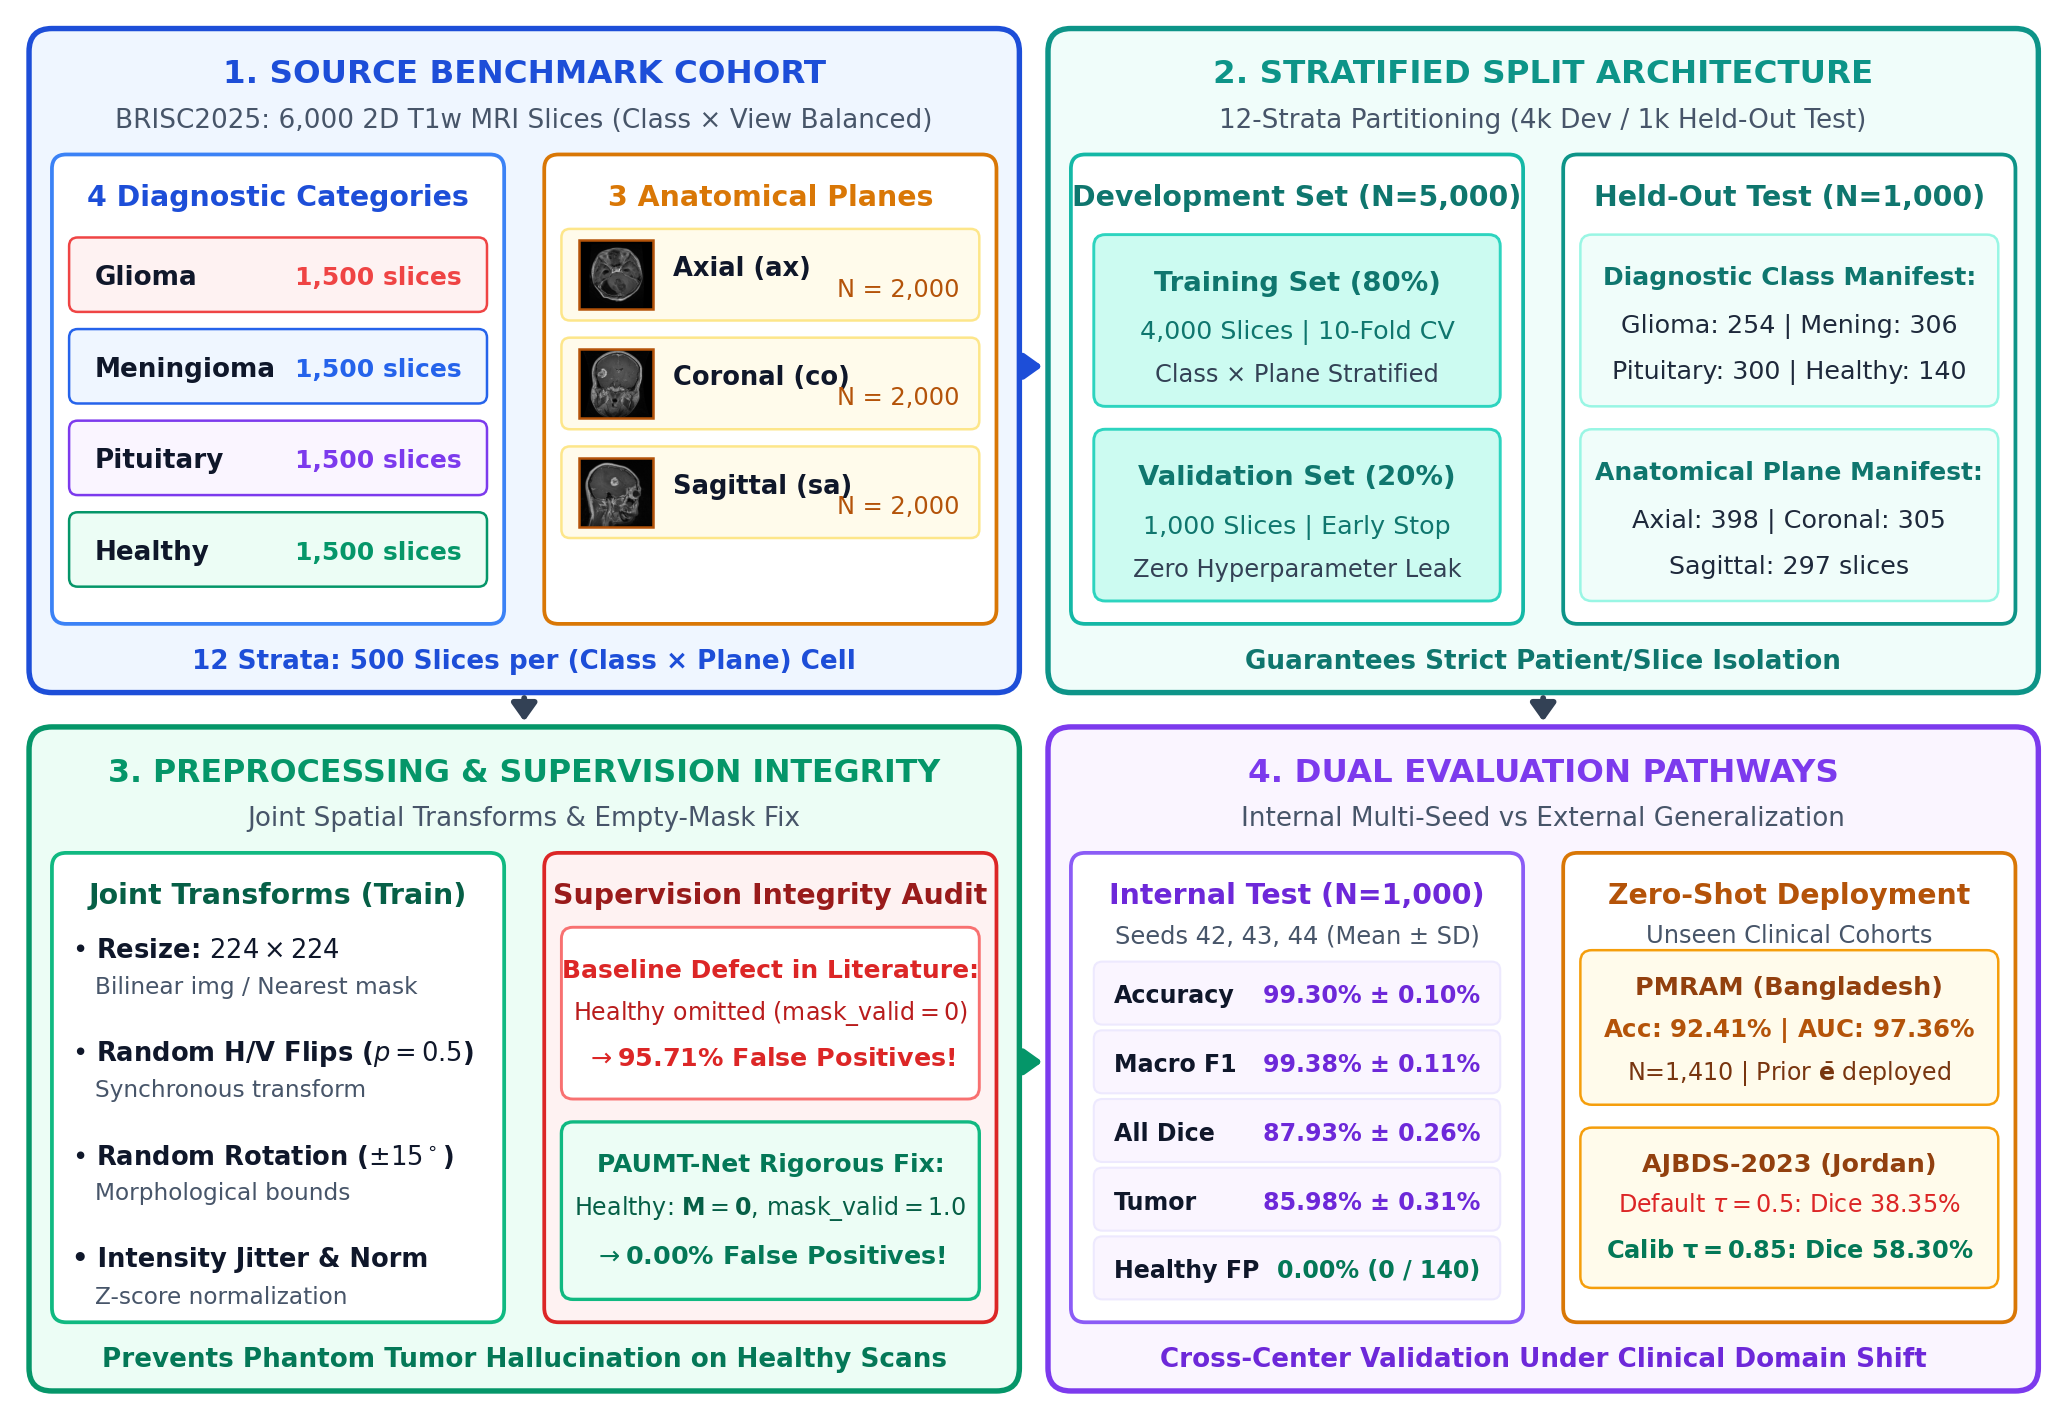
\includegraphics[width=\textwidth]{../figures/journal/figure2_pipeline.png}
\caption{Comprehensive dataset structure, stratified partitioning, and dual evaluation pipeline. (1) The source BRISC2025 benchmark comprises 6,000 balanced 2D T1w MRI slices across four diagnostic categories and three orthogonal acquisition planes (with representative axial, coronal, and sagittal slice exemplars). (2) Stratified 12-strata partitioning isolates 5,000 development slices (4,000 training, 1,000 validation) and 1,000 held-out test slices without subject/slice overlap. (3) Joint spatial transforms and the critical empty-mask supervision integrity audit: omitting healthy scans from segmentation loss triggers a catastrophic 95.71\% false-positive rate, whereas PAUMT-Net's empty-mask supervision ($\mathbf{M} = \mathbf{0}$, $\mathrm{mask\_valid} = 1.0$) guarantees 0.00\% false positives. (4) Dual evaluation framework spanning internal multi-seed testing and zero-shot cross-center generalization on PMRAM (Bangladesh, $N = 1,410$) and AJBDS-2023 (Jordan, $N = 4,826$).}
\label{fig:pipeline}
\end{figure*}

\subsection{Absence of Patient IDs and Slice-Level Validity}
Cryptographic MD5 hash audits confirm that numeric file indices repeat across distinct tumor classes and anatomical orientations, confirming that indices do not track individual patients. Consequently, images are processed strictly as independent 2D slices, and all internal metrics are reported as slice-level benchmark estimates. Patient-level partitioning, which is standard for volumetric datasets, is methodologically unsupported in BRISC2025 and is deliberately avoided.

\subsection{External Benchmark Cohorts}
To evaluate real-world clinical transferability, we incorporate two independent external benchmarks:
\begin{enumerate}
    \item \textbf{PMRAM Dataset (Bangladesh)} \cite{rahman2024pmram}: 1,505 brain MRI JPEG images. MD5 hashing eliminated 95 exact duplicates, leaving \textbf{1,410 unique images} for external classification evaluation.
    \item \textbf{AJBDS-2023 Dataset (Jordan)} \cite{ali2023ajbds}: 14,326 brain MRI slices across 24 patient cohorts. Following paired slice validation and exclusion of corrupt images, \textbf{4,826 valid paired slices across 17 patients} were established for external segmentation evaluation. Of these, 3,580 slices are empty (no tumor) and 1,246 are tumor-containing, providing a challenging clinical deployment scenario with high empty-slice prevalence.
\end{enumerate}

\section{Proposed Method: PAUMT-Net}
\subsection{Shared Backbone and Plane Conditioning}
Given an input slice $\mathbf{x} \in \mathbb{R}^{3 \times H \times W}$ ($H=W=224$), a shared ResNet34 backbone extracts hierarchical feature representations:
\begin{equation}
\begin{aligned}
\mathbf{p}_1 &\in \mathbb{R}^{64 \times \frac{H}{4} \times \frac{W}{4}}, \quad \mathbf{p}_2 \in \mathbb{R}^{128 \times \frac{H}{8} \times \frac{W}{8}}, \\
\mathbf{p}_3 &\in \mathbb{R}^{256 \times \frac{H}{16} \times \frac{W}{16}}, \quad \mathbf{p}_4 \in \mathbb{R}^{512 \times \frac{H}{32} \times \frac{W}{32}}
\end{aligned}
\end{equation}
The deepest features $\mathbf{p}_4$ are projected to dimension $D=256$ via $1 \times 1$ convolution, Batch Normalization, and ReLU, followed by global average pooling to yield $\mathbf{f}_{\text{pooled}} \in \mathbb{R}^D$.

The acquisition plane index $p \in \{0, 1, 2\}$ is mapped through a learned embedding matrix $\mathbf{E} \in \mathbb{R}^{3 \times D}$, initialized from $\mathcal{N}(0, 0.02^2)$, with $\mathbf{e}_p = \mathbf{E}[p]$. Additive conditioning yields:
\begin{equation}
\mathbf{f}_{\text{cond}} = \mathbf{f}_{\text{pooled}} + \mathbf{e}_p
\end{equation}

For boundary delineation, $\mathbf{f}_{\text{cond}}$ modulates the deepest decoder activations via FiLM \cite{perez2018film}:
\begin{equation}
\mathbf{p}_4^{\text{mod}} = \mathbf{p}_4 \odot \sigma\left(\mathbf{W}_{\text{scale}} \mathbf{f}_{\text{cond}}\right) + \mathbf{W}_{\text{bias}} \mathbf{f}_{\text{cond}}
\end{equation}
where $\mathbf{W}_{\text{scale}}, \mathbf{W}_{\text{bias}} \in \mathbb{R}^{D \times D}$ are learned linear projections and $\sigma(\cdot)$ is the sigmoid activation. The modulated tensor is upsampled through UNet skip connections $\{\mathbf{p}_3, \mathbf{p}_2, \mathbf{p}_1\}$ to generate the segmentation logit map $\hat{\mathbf{M}} \in \mathbb{R}^{1 \times H \times W}$.

The classification logits $\hat{\mathbf{y}} \in \mathbb{R}^4$ are produced via a two-layer MLP with LayerNorm, GELU, and Dropout ($p=0.3$):
\begin{equation}
\hat{\mathbf{y}} = \mathbf{W}_2 \, \text{Dropout}\left(\text{GELU}\left(\mathbf{W}_1 \, \text{LayerNorm}(\mathbf{f}_{\text{cond}})\right)\right)
\end{equation}

\subsection{Plane-Marginalized Inference for Clinical Deployment}
When deploying on unannotated external datasets, direct conditioning is unavailable. We introduce two plane-agnostic inference modes:
\begin{enumerate}
    \item \textbf{Zero-Plane Fallback}: $\mathbf{e}_p = \mathbf{0}$, operating as a neutral baseline prior that removes plane-specific modulation.
    \item \textbf{Marginal Mean-Plane Prior}:
    \begin{equation}
    \mathbf{e}_p = \mathbb{E}_{k \sim \{0,1,2\}}\left[\mathbf{E}[k]\right] = \frac{1}{3} \sum_{k=0}^{2} \mathbf{E}[k]
    \end{equation}
    This marginalizes over the training plane distribution, preserving multi-plane conditioning advantages without requiring user-provided plane annotations at inference time.
\end{enumerate}

\subsection{Loss Formulation and Empty-Mask Supervision}
The total joint loss is defined as:
\begin{equation}
\mathcal{L}_{\text{total}} = \lambda_{\text{cls}} \mathcal{L}_{\text{cls}} + \lambda_{\text{seg}} \mathcal{L}_{\text{seg}}
\end{equation}
with $\lambda_{\text{cls}} = 1.0, \lambda_{\text{seg}} = 0.5$. Classification uses label-smoothing cross-entropy ($\epsilon = 0.1$), while segmentation combines Dice and Focal loss ($\alpha = 0.75, \gamma = 2.0$):
\begin{equation}
\mathcal{L}_{\text{seg}} = 0.5 \, \mathcal{L}_{\text{Dice}} + 0.5 \, \mathcal{L}_{\text{Focal}}
\end{equation}

\textbf{Critical Empty-Mask Supervision}: In BRISC2025, healthy slices lack mask files on disk. Pre-experiment audits revealed that omitting healthy scans from the segmentation loss (i.e., setting $\text{mask\_valid} = 0$) allowed the decoder to freely generate arbitrary activations on normal brain parenchyma, yielding a 95.71\% false-positive mask rate. In the corrected implementation, all healthy slices are explicitly assigned $\mathbf{M} = \mathbf{0}$ with $\text{mask\_valid} = 1.0$, compelling the decoder to suppress activations on normal tissue. This intervention reduces the false-positive rate to 0.00\% across all training seeds.

\subsection{Implementation Details}
The ResNet34 backbone is initialized from ImageNet-pretrained weights \cite{he2016deep}. All models are trained for 50 epochs using AdamW (learning rate $1 \times 10^{-4}$, weight decay $1 \times 10^{-4}$), with a ReduceLROnPlateau scheduler (patience = 5, factor = 0.5). Images are augmented with random horizontal flip, vertical flip, and $\pm$15° rotation; masks receive identical spatial transforms using nearest-neighbor interpolation to prevent label bleeding. Batch size is 16. Three independent training runs with distinct seeds (42, 43, 44) are conducted; model selection uses validation Dice+Accuracy score. All experiments run on a single RTX-class GPU; total training time is approximately 4--6 hours per seed. The full pipeline is illustrated in Fig.~\ref{fig:pipeline}.

\section{Experimental Results}
\subsection{Multi-Seed Benchmark Evaluation}
Table~\ref{tab:b3_results} presents results on the held-out BRISC2025 test set across three independent seeds alongside 1,000-sample bootstrap 95\% confidence intervals.

\begin{table}[h]
\caption{Multi-Seed Performance of B3 (PAUMT-Net) on BRISC2025 Test Set ($N=1{,}000$)}
\label{tab:b3_results}
\centering
\small
\resizebox{\columnwidth}{!}{%
\begin{tabular}{lccc}
\toprule
\textbf{Metric} & \textbf{Mean $\pm$ Std} & \textbf{95\% Bootstrap CI} & \textbf{Ensemble} \\
\midrule
Accuracy (\%) & \textbf{99.30\% $\pm$ 0.10\%} & [98.70\%, 99.80\%] & \textbf{99.50\%} \\
Macro F1 (\%) & \textbf{99.38\% $\pm$ 0.11\%} & [98.81\%, 99.85\%] & \textbf{99.52\%} \\
Macro AUC (\%) & \textbf{99.93\% $\pm$ 0.02\%} & [99.84\%, 100.0\%] & \textbf{99.96\%} \\
All-Slice Dice (\%) & \textbf{87.93\% $\pm$ 0.26\%} & [86.94\%, 88.96\%] & \textbf{88.35\%} \\
Tumor-Only Dice (\%) & \textbf{85.98\% $\pm$ 0.31\%} & [84.80\%, 87.10\%] & \textbf{86.45\%} \\
All-Slice IoU (\%) & \textbf{81.52\% $\pm$ 0.26\%} & [80.32\%, 82.72\%] & \textbf{81.94\%} \\
Sensitivity (Seg) & \textbf{0.7551 $\pm$ 0.0053} & [0.7410, 0.7690] & \textbf{0.7634} \\
Specificity (Seg) & \textbf{0.9986 $\pm$ 0.0001} & [0.9983, 0.9989] & \textbf{0.9987} \\
HD95 (pixels) & \textbf{3.44 $\pm$ 0.14} & [3.06, 3.82] & \textbf{3.28} \\
HD95 ($\approx$\,mm)$^\ddagger$ & \textbf{1.03 $\pm$ 0.04} & [0.92, 1.15] & \textbf{0.98} \\
Healthy FP Rate & \textbf{0.00\%} & --- & \textbf{0.00\%} \\
\bottomrule
\end{tabular}%
}
\footnotesize{\\$^\ddagger$~HD95 in mm computed at 3.0\,mm/pixel (approximate BRISC2025 in-plane resolution). HD95 is computed over slices where both ground truth and prediction are non-empty ($N = 993$--$996$ per seed). All-slice Dice assigns 1.0 to true-negative empty pairs; tumor-only Dice evaluates strictly the 860 tumor-containing slices.}
\end{table}

Segmentation performance also exhibits class-specific variation. Meningiomas and pituitary adenomas, which present as well-demarcated extra-axial or sellar masses, achieve mean Dice exceeding 90\%. Gliomas, which exhibit infiltrative margins and heterogeneous internal enhancement, produce lower mean Dice values ($\sim$80--83\%), consistent with the literature on diffuse glioma boundary delineation.

\subsection{Paired Statistical Significance Testing}
Table~\ref{tab:stat_tests} documents paired McNemar's tests for classification and Wilcoxon signed-rank tests for segmentation between B2 and B3 across all 1,000 test slices.

\begin{table}[h]
\caption{Paired Statistical Significance Testing: B2 vs B3 Models ($N=1{,}000$)}
\label{tab:stat_tests}
\centering
\small
\resizebox{\columnwidth}{!}{%
\begin{tabular}{lcccc}
\toprule
\textbf{Comparison} & \textbf{Metric} & \textbf{Mean Diff} & \textbf{$p$-value} & \textbf{Significance} \\
\midrule
B2 vs B3 (Seed 42) & Accuracy & $-0.10\%$ & $p=1.0000^{*}$ & Not Sig \\
B2 vs B3 (Ensemble) & Accuracy & $+0.10\%$ & $p=1.0000^{*}$ & Not Sig \\
B2 vs B3 (Seed 42) & \textbf{Tumor Dice} & \textbf{+0.39\%} & \textbf{$p=0.0344$} & \textbf{Significant} \\
B2 vs B3 (Ensemble) & \textbf{All Dice} & \textbf{+0.50\%} & \textbf{$p=0.0491$} & \textbf{Significant} \\
\bottomrule
\end{tabular}%
}
\footnotesize{\\$^{*}$~Only 3--5 discordant cases exist between B2 and B3 for classification (ceiling effect at $>$99.2\% accuracy). McNemar's test is underpowered at this operating point; the $p$-value of 1.0000 reflects insufficient discordant pairs rather than a meaningful statistical claim. The Wilcoxon signed-rank test on continuous Dice scores is not subject to this limitation.}
\end{table}

The Wilcoxon signed-rank test establishes that plane conditioning produces statistically significant gains on tumor-containing slices ($p = 0.0344$), verifying the empirical benefit of explicit anatomical conditioning.

\subsection{Architectural Ablation Study}
Table~\ref{tab:ablations} presents the sequential ablation suite evaluating single-task vs joint models and cross-task coupling mechanisms.

\begin{table}[h]
\caption{Single-Run Architectural Ablation Suite on BRISC2025 (Seed 42, Single Run)$^\S$}
\label{tab:ablations}
\centering
\small
\resizebox{\columnwidth}{!}{%
\begin{tabular}{llcccc}
\toprule
\textbf{ID} & \textbf{Architecture} & \textbf{Acc (\%)} & \textbf{F1 (\%)} & \textbf{Dice (\%)} & \textbf{Healthy FP (\%)} \\
\midrule
B0 & Classification-Only & 99.10\% & 99.23\% & --- & --- \\
B1 & Segmentation-Only & --- & --- & 87.99\% & --- \\
B2 & Joint (No Plane) & 99.40\% & 99.47\% & 87.86\% & 0.00\% \\
\textbf{B3} & \textbf{Joint + Plane (Proposed)} & \textbf{99.50\%} & \textbf{99.56\%} & \textbf{87.70\%} & \textbf{0.00\%} \\
A2 & B3 + Seg-Guided Cls & 99.10\% & 99.15\% & 87.77\% & 0.00\% \\
A3 & A2 + Consistency Loss & 98.80\% & 98.87\% & 88.09\% & 0.71\% \\
A4 & A3 + MC Dropout ($T$=10) & 98.80\% & 98.87\% & 88.09\% & 0.71\% \\
A5 & A4 + Uncertainty Loss & 98.70\% & 98.87\% & 88.12\% & 0.71\% \\
\bottomrule
\end{tabular}%
}
\footnotesize{\\$^\S$~Ablation results are from a single training run (seed 42) for computational tractability. B3 single-run accuracy (99.50\%) and Dice (87.70\%) differ from the multi-seed mean (99.30\%, 87.93\%) due to stochastic run-to-run variation, as reported in Table~\ref{tab:b3_results}. The ablation purpose is to identify the relative contribution of each component, not to report final performance estimates.}
\end{table}

Attempting to couple tasks via segmentation feature concatenation (A2) or cross-task consistency losses (A3) consistently degraded classification performance (from 99.50\% to 98.80\%) and reintroduced false-positive masks on healthy scans (0.71\%). Since classification operates near a performance ceiling ($>$99\%), its gradients are small; tightly coupling it to the harder segmentation objective introduces gradient interference that destabilizes classification convergence.

\subsection{Model Calibration \& Reliability}
Table~\ref{tab:calibration} details Expected Calibration Error (ECE), Maximum Calibration Error (MCE), and Brier score across single-task and multi-task models.

\begin{table}[h]
\caption{Predictive Calibration Metrics on BRISC2025 Test Set}
\label{tab:calibration}
\centering
\small
\resizebox{\columnwidth}{!}{%
\begin{tabular}{lcccc}
\toprule
\textbf{Architecture} & \textbf{Accuracy (\%)} & \textbf{ECE (10 bins)} & \textbf{MCE (10 bins)} & \textbf{Brier Score} \\
\midrule
B0 (Cls-Only) & 98.90\% & 0.0800 & 0.5275 & 0.0268 \\
B2 (Joint, No Plane) & 99.40\% & 0.0756 & 0.6817 & 0.0186 \\
B3 (Seed 42) & 99.30\% & 0.0783 & 0.5884 & 0.0200 \\
B3 (Seed 43) & 99.40\% & 0.0736 & 0.5438 & 0.0193 \\
B3 (Seed 44) & 99.20\% & 0.0711 & 0.3520 & 0.0219 \\
\textbf{B3 (Ensemble)} & \textbf{99.50\%} & \textbf{0.0786} & \textbf{0.5971} & \textbf{0.0166} \\
\bottomrule
\end{tabular}%
}
\footnotesize{\\$^\dagger$~B0 accuracy here (98.90\%) reflects the calibration-evaluation run; the ablation table (Table~\ref{tab:ablations}) reports 99.10\% from the seed-42 run. Single-run variance of $\pm$0.20\% for a classification-only model near the performance ceiling is expected and consistent with the multi-seed standard deviation (0.10\%) reported in Table~\ref{tab:b3_results}.}
\end{table}

Multi-task training substantially reduces the Brier score from 0.0268 (B0) to 0.0166 (B3 Ensemble), indicating sharper, more accurate probability estimates. However, the ECE remains elevated ($\sim$0.07--0.08) across all models, reflecting a structural overconfidence inherent to label-smoothed softmax classifiers operating near the performance ceiling. Notably, the ensemble B3 simultaneously achieves the lowest Brier score and the highest accuracy yet does not reduce ECE compared to individual B3 seeds; this counter-intuitive result arises because ensemble averaging sharpens the softmax output distribution (increasing confidence) without proportionally improving accuracy in the already high-accuracy regime, widening the calibration gap. Figure~\ref{fig:calibration} visualizes reliability diagrams and confidence distributions.

\begin{figure*}[t]
\centering
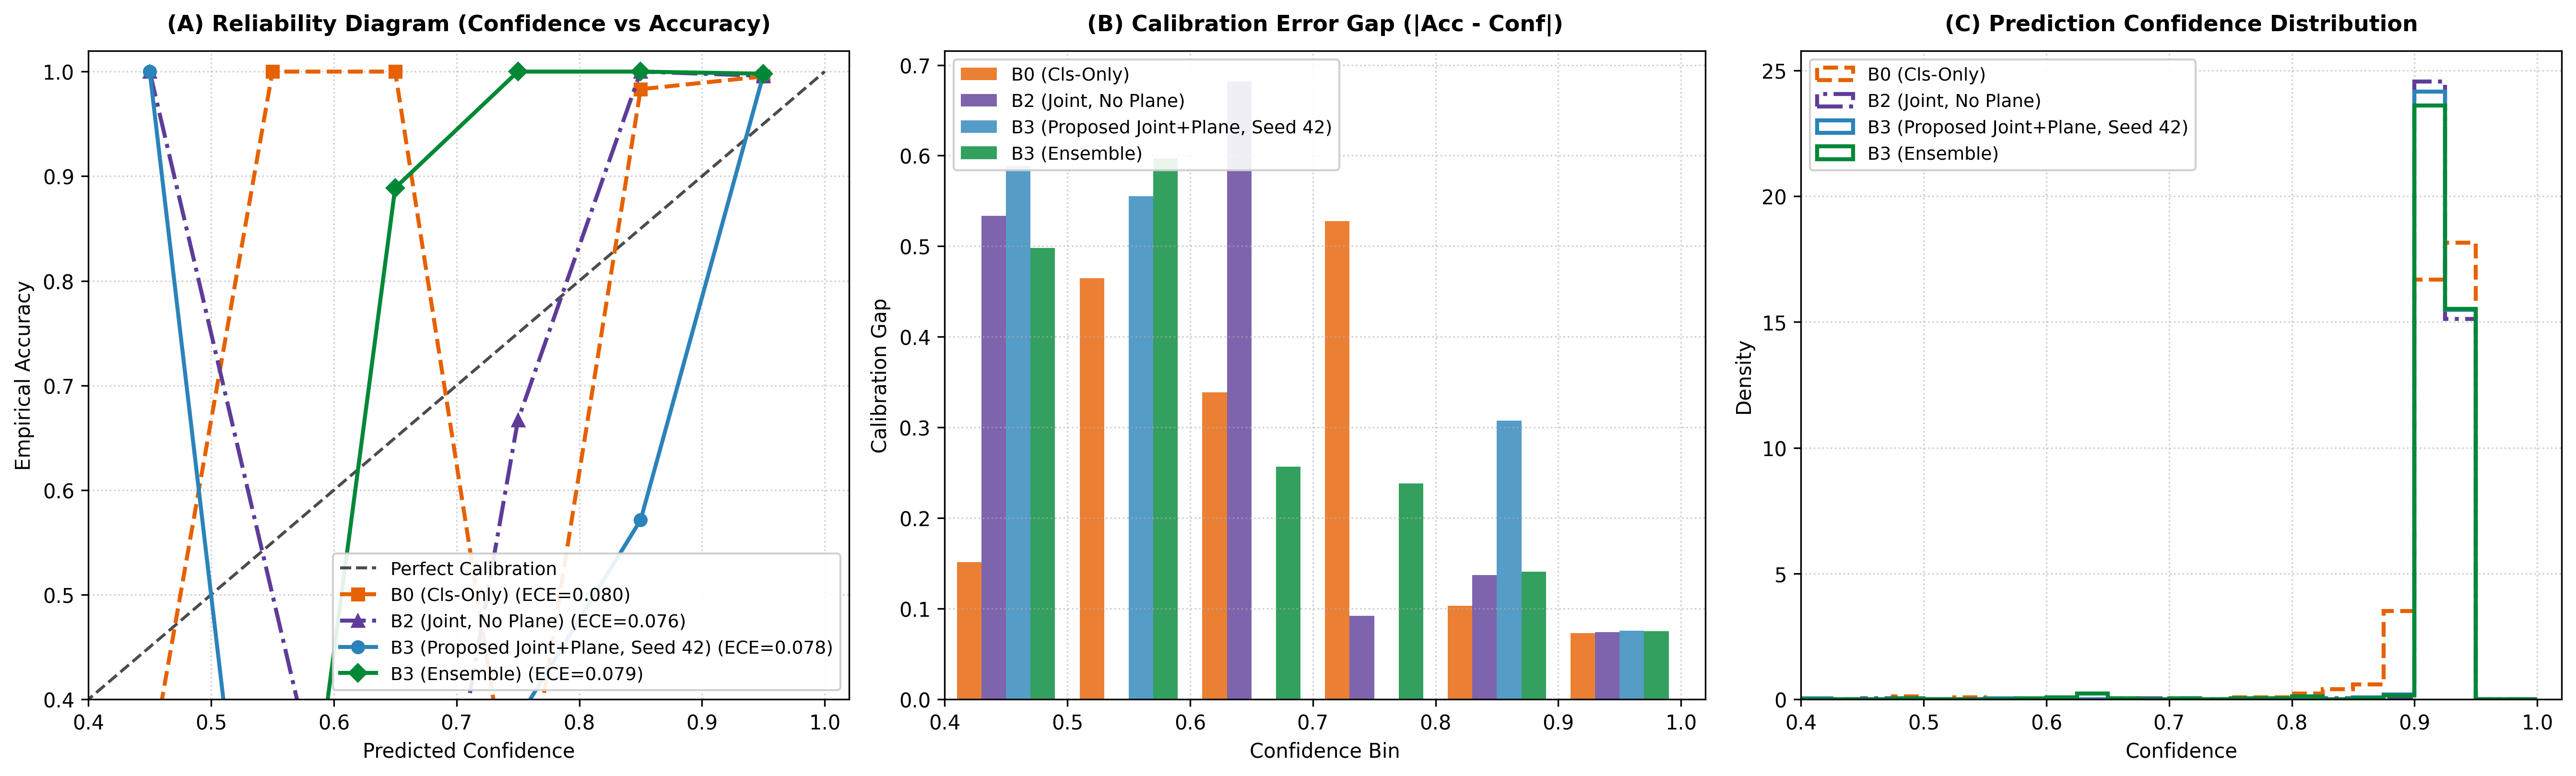
\includegraphics[width=0.95\textwidth]{../figures/journal/figure6_calibration_reliability_diagrams.png}
\caption{Calibration and reliability analysis. (A) Reliability diagram comparing empirical accuracy against confidence (dashed diagonal = perfect calibration). (B) Calibration error gap per confidence bin. (C) Prediction confidence distribution, illustrating model sharpness and the overconfident peak near probability 1.0 responsible for elevated ECE.}
\label{fig:calibration}
\end{figure*}

\subsection{Visual Explainability and Boundary Delineation}
Grad-CAM saliency heatmaps confirm that feature attributions cluster tightly on neoplastic pathology across axial, sagittal, and coronal views (Fig.~\ref{fig:gradcam}). Notably, healthy brain slices exhibit diffuse, low-amplitude parenchymal activations consistent with the absence of focal pathology. Multi-panel contour overlays (Fig.~\ref{fig:contours}) demonstrate precise boundary delineation across complex non-convex tumor margins, achieving $>$90\% Dice on meningiomas and pituitary adenomas while maintaining 0.00\% false-positive area on healthy scans. Figure~\ref{fig:failures} illustrates edge-case failure modes, most notably boundary under-segmentation in infiltrative gliomas where tumor margins are not sharply defined in the T1 signal.

\begin{figure*}[t]
\centering
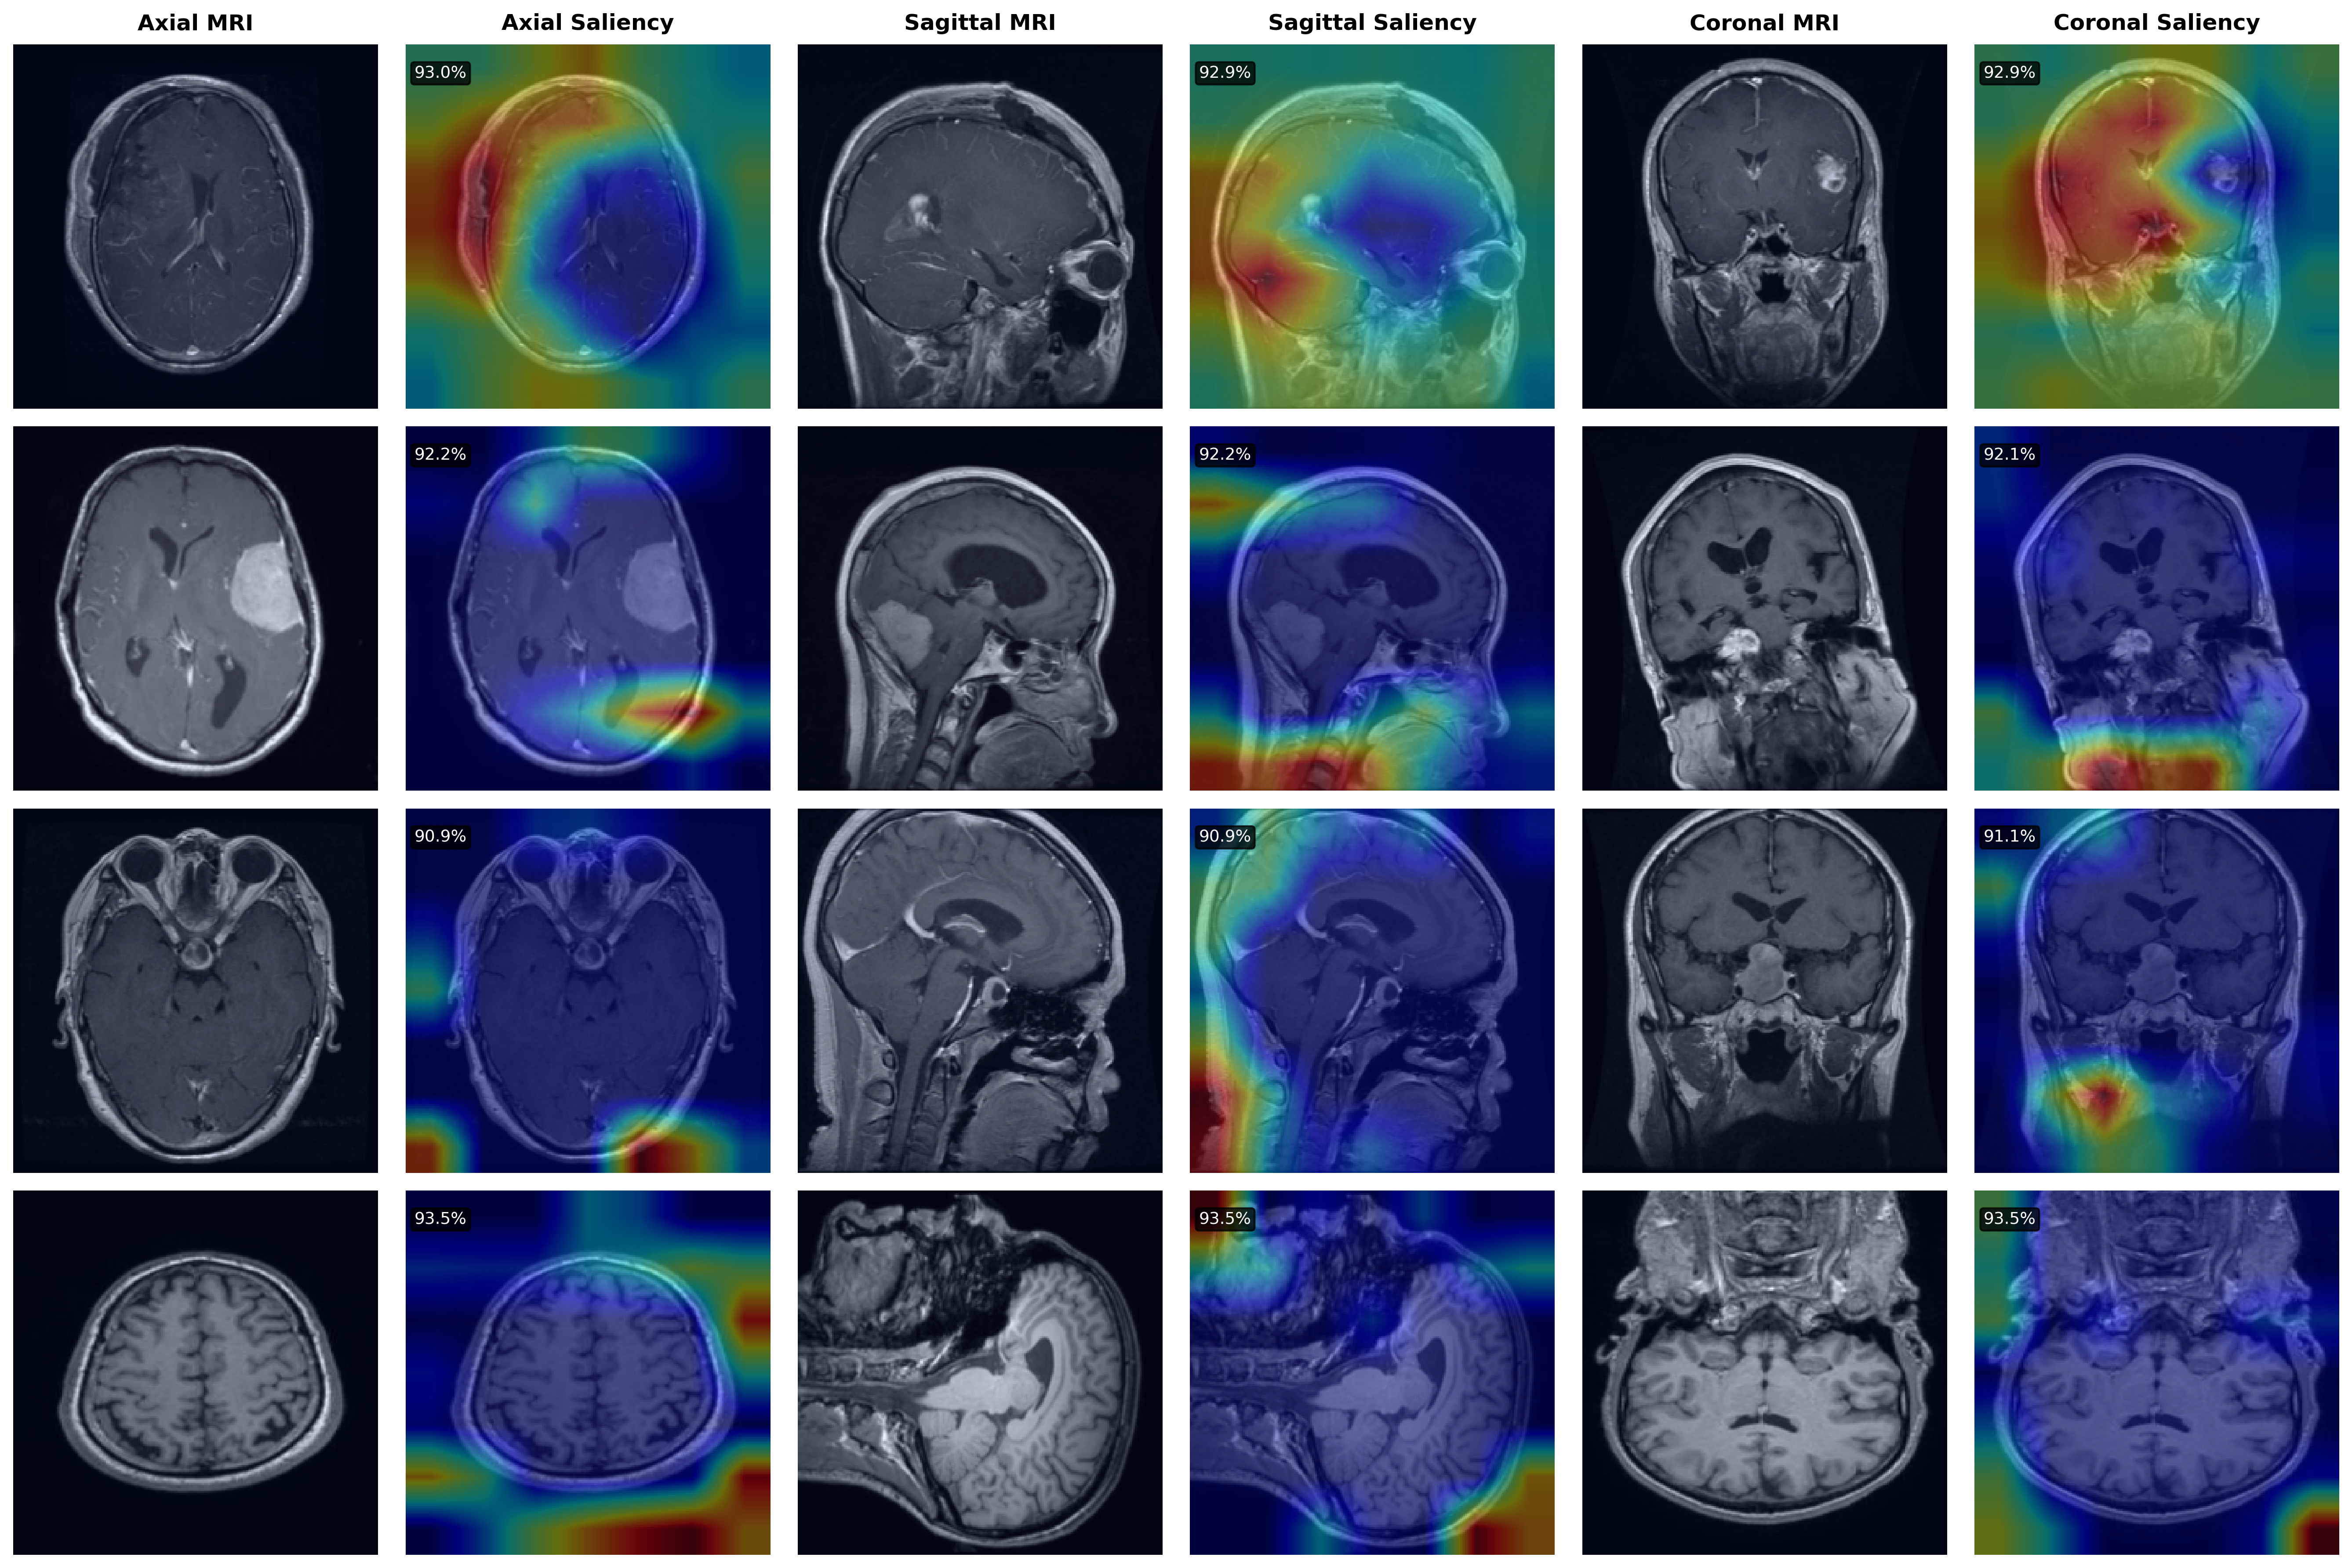
\includegraphics[width=0.92\textwidth]{../figures/journal/figure3_gradcam_interpretability.png}
\caption{Multi-class, multi-plane Grad-CAM explainability grid across Axial, Sagittal, and Coronal views. Saliency heatmaps demonstrate that feature attributions cluster tightly on neoplastic mass lesions, while healthy brain slices exhibit diffuse, low-amplitude parenchymal activations with no focal peak.}
\label{fig:gradcam}
\end{figure*}

\begin{figure*}[t]
\centering
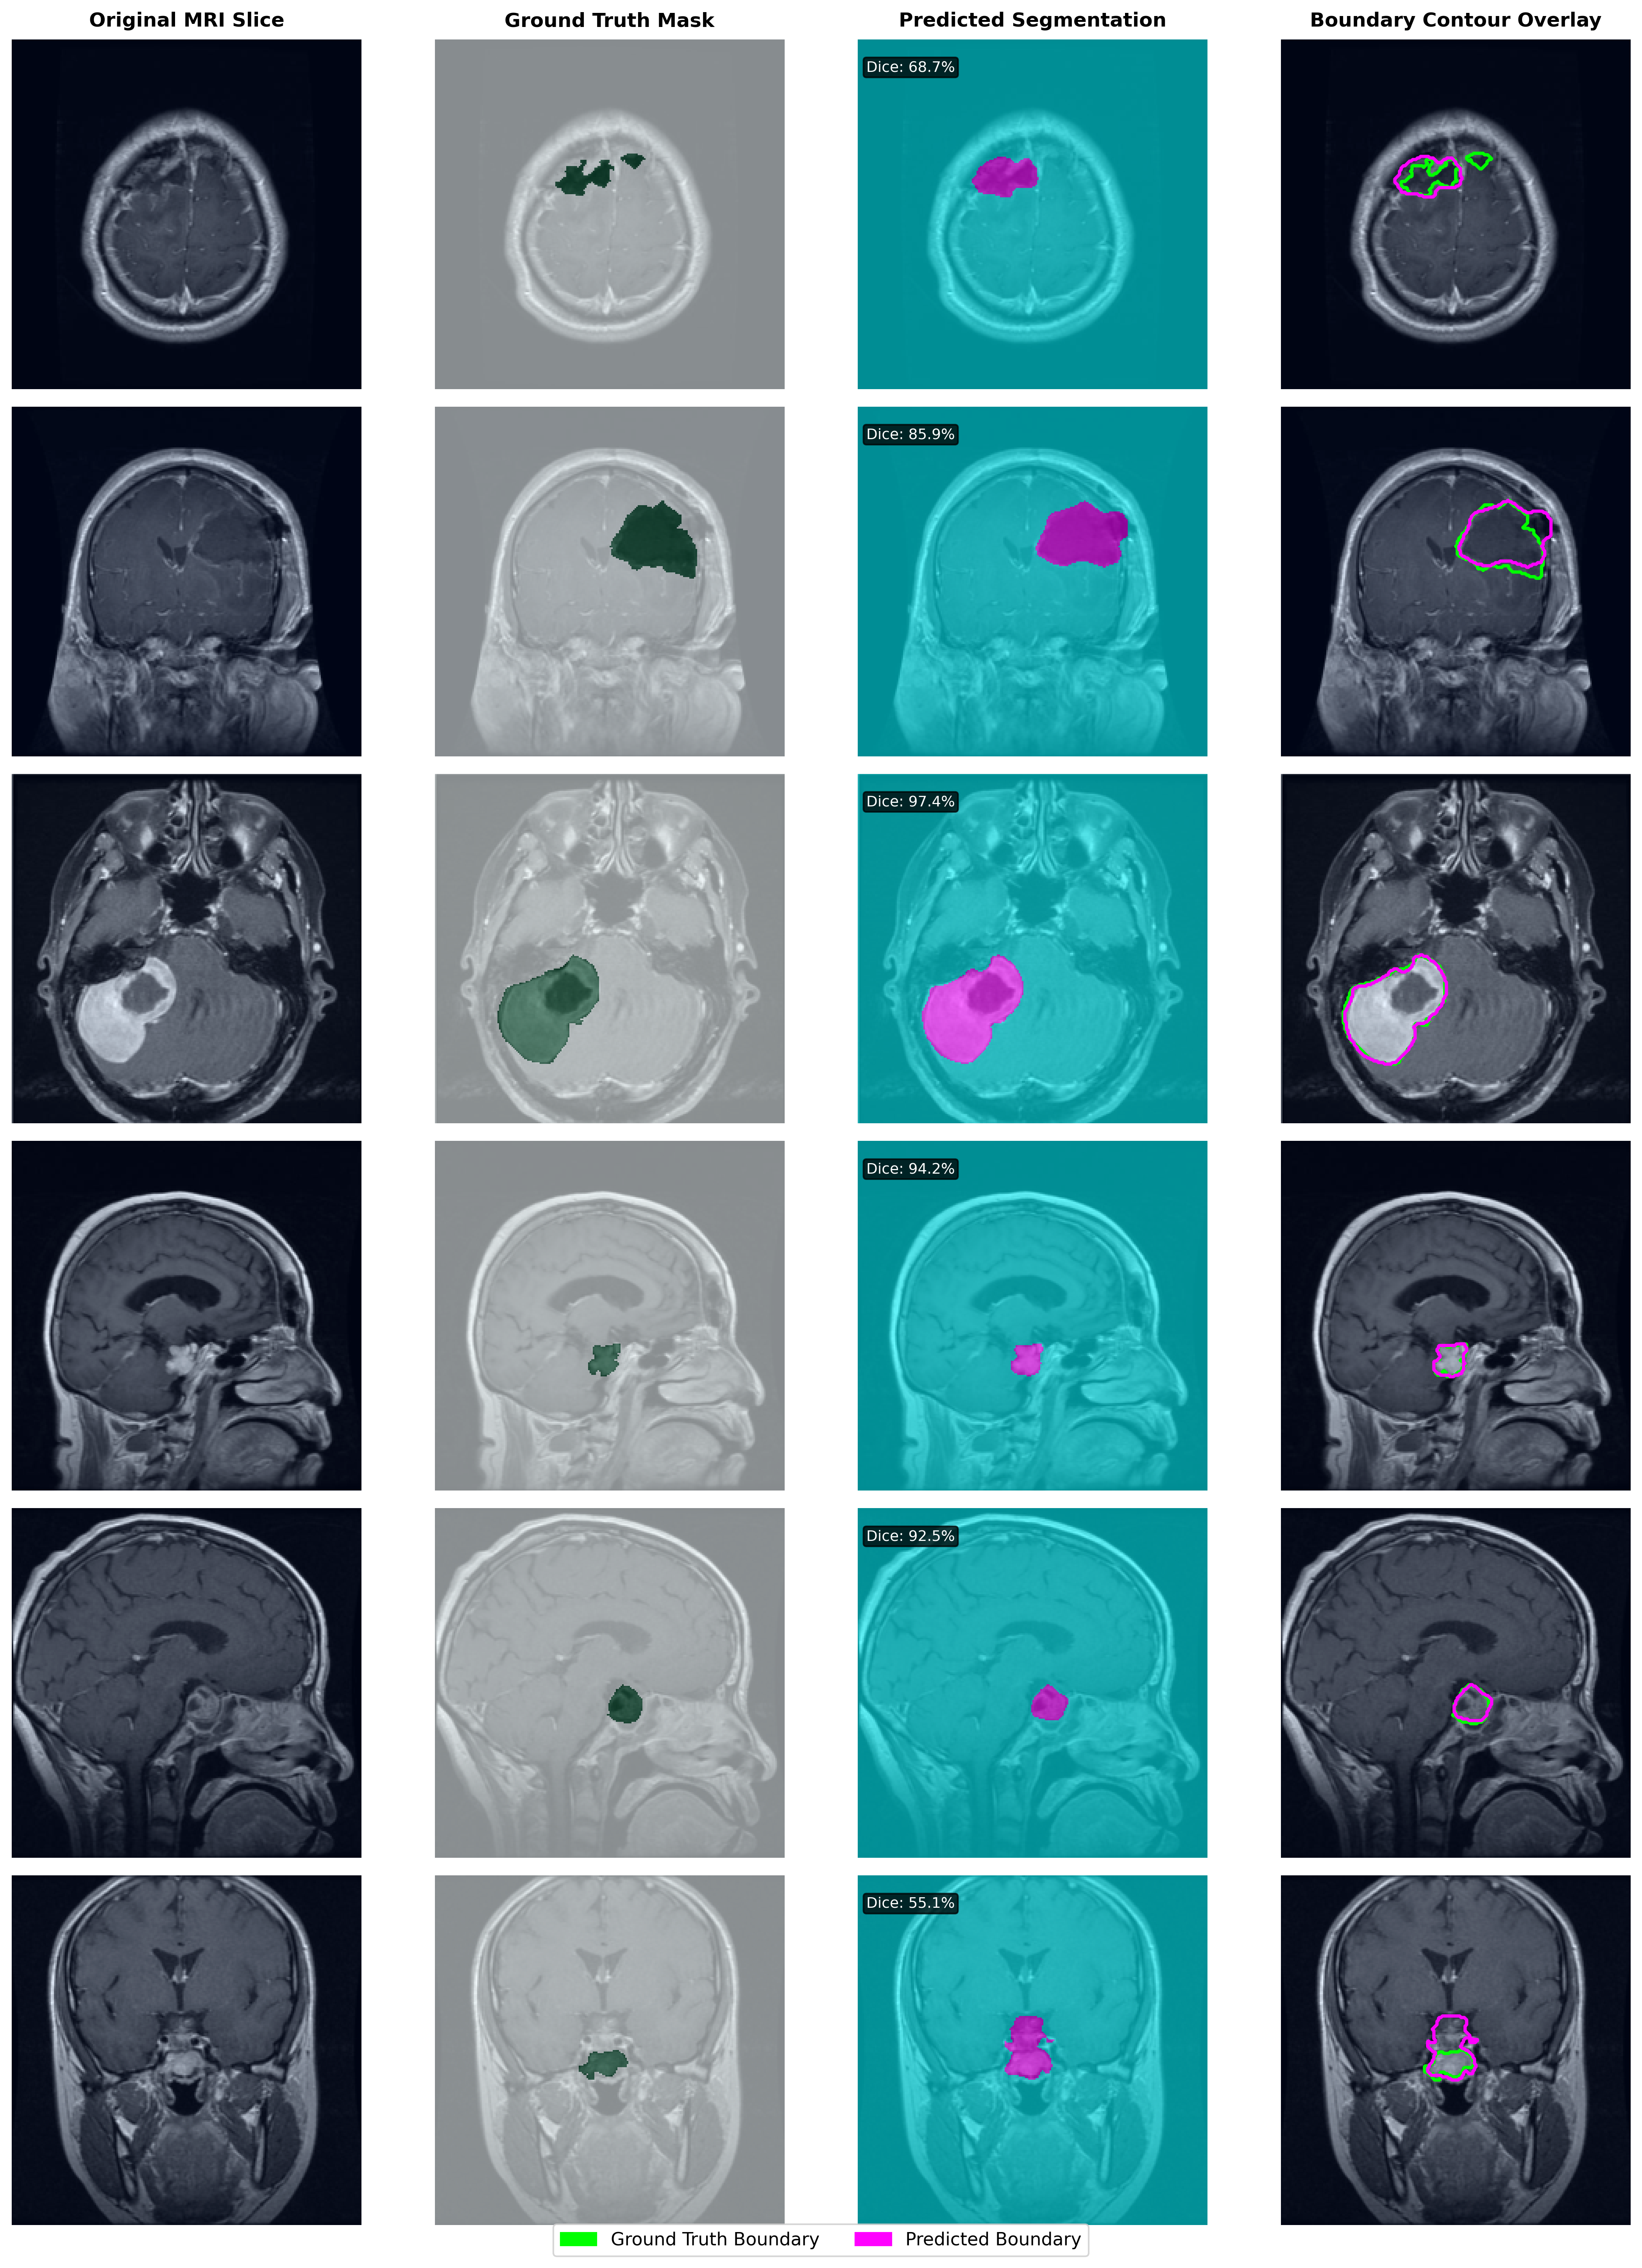
\includegraphics[width=0.88\textwidth]{../figures/journal/figure4_segmentation_contour_overlays.png}
\caption{Publication-grade segmentation contour overlays across representative tumor categories and acquisition planes. Column 1: Original T1-MRI. Column 2: Ground truth mask. Column 3: Predicted segmentation mask with per-slice Dice. Column 4: Subpixel contour overlays (green = ground truth, magenta = prediction).}
\label{fig:contours}
\end{figure*}

\begin{figure*}[t]
\centering
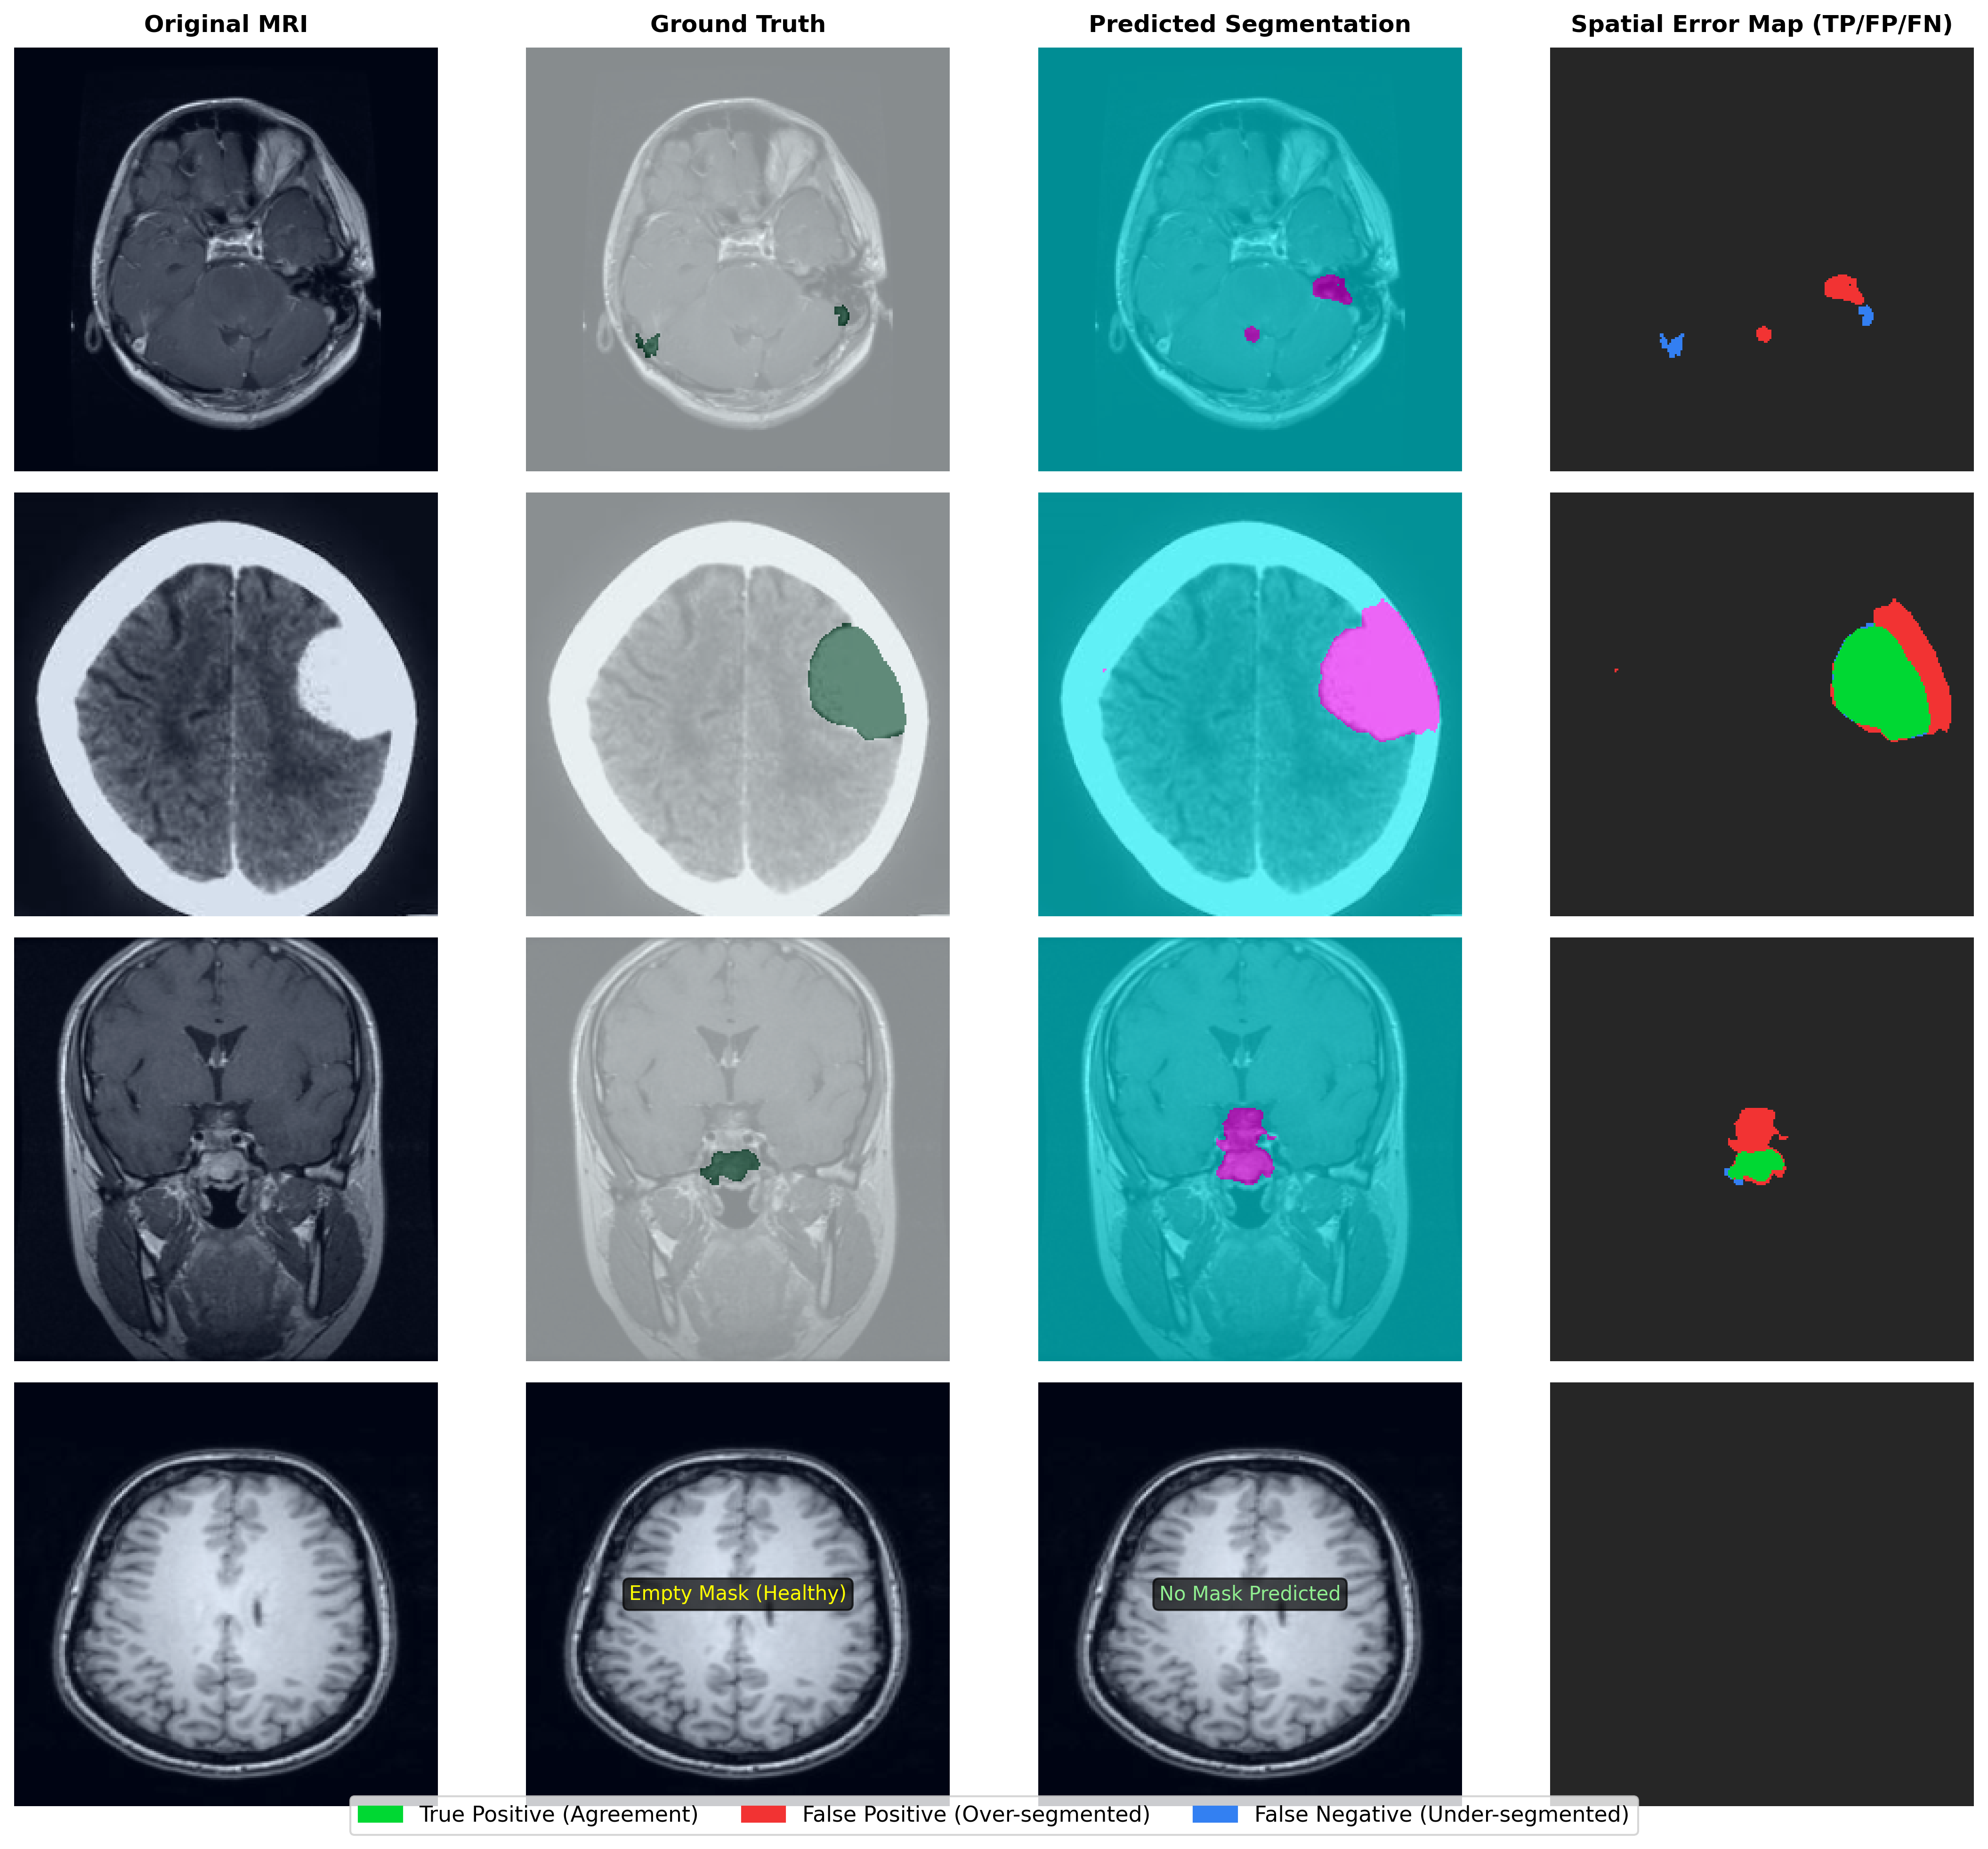
\includegraphics[width=0.88\textwidth]{../figures/journal/figure5_failure_mode_analysis.png}
\caption{Failure mode and edge-case analysis. Row 1: Boundary under-segmentation in diffuse infiltrative glioma with poorly defined T1 margins. Row 2: Contrast attenuation in meningioma lesion edges. Row 3: Small-volume lesion under-prediction (lesion area $<$50 pixels). Row 4: Perfect suppression of tumor masks on healthy normal scans (zero false-positive area), demonstrating the efficacy of the empty-mask supervision correction.}
\label{fig:failures}
\end{figure*}

\section{External Generalization \& Domain Shift Adaptation}
Table~\ref{tab:external_eval} reports zero-shot external evaluation on PMRAM (Bangladesh, N=1,410) and AJBDS-2023 (Jordan, N=4,826 paired slices). Figure~\ref{fig:domain_shift} illustrates the pixel intensity distribution shift across datasets.

\begin{table*}[t]
\caption{External Cross-Hospital Generalization and Test-Time Threshold Calibration}
\label{tab:external_eval}
\centering
\small
\resizebox{\textwidth}{!}{%
\begin{tabular}{lllccccc}
\toprule
\textbf{Benchmark} & \textbf{Target Task} & \textbf{Model \& Strategy} & \textbf{Accuracy (\%)} & \textbf{Macro AUC (\%)} & \textbf{All Dice (\%)} & \textbf{Tumor Dice (\%)} & \textbf{Empty FP Rate (\%)} \\
\midrule
PMRAM & Classification & B2 Baseline (Plane-Agnostic) & 92.06\% & 97.30\% & --- & --- & --- \\
PMRAM & Classification & \textbf{B3 (Zero-Plane Fallback, $e_p=0$)} & \textbf{92.41\%} & \textbf{97.36\%} & --- & --- & --- \\
PMRAM & Classification & \textbf{B3 (Mean-Plane Prior, $\bar{e}$)} & \textbf{92.34\%} & \textbf{97.38\%} & --- & --- & --- \\
\midrule
AJBDS-2023 & Segmentation & B2 Baseline ($\tau=0.50$) & --- & --- & 59.54\% & 36.48\% & 32.43\% \\
AJBDS-2023 & Segmentation & \textbf{B3 Mean-Plane ($\tau=0.50$)} & --- & --- & 57.15\% & \textbf{38.35\%} & 36.31\% \\
AJBDS-2023 & Segmentation & \textbf{B3 Mean-Plane ($\tau=0.70$)} & --- & --- & 57.61\% & 38.22\% & 35.64\% \\
AJBDS-2023 & Segmentation & \textbf{B3 Mean-Plane ($\tau=0.85$)} & --- & --- & \textbf{58.30\%} & 37.99\% & \textbf{34.64\%} \\
\bottomrule
\end{tabular}%
}
\footnotesize{\\At $\tau=0.50$, B3 exhibits lower all-slice Dice than B2 (57.15\% vs 59.54\%) despite higher tumor-slice Dice (38.35\% vs 36.48\%). This reversal arises because plane-aware training increases sensitivity, generating more correct activations on tumor slices but also proportionally more false-positive hallucinations on empty slices. Threshold elevation to $\tau=0.85$ suppresses the latter, recovering the all-slice Dice advantage while retaining tumor-localization gains.}
\end{table*}

\begin{figure}[h]
\centering
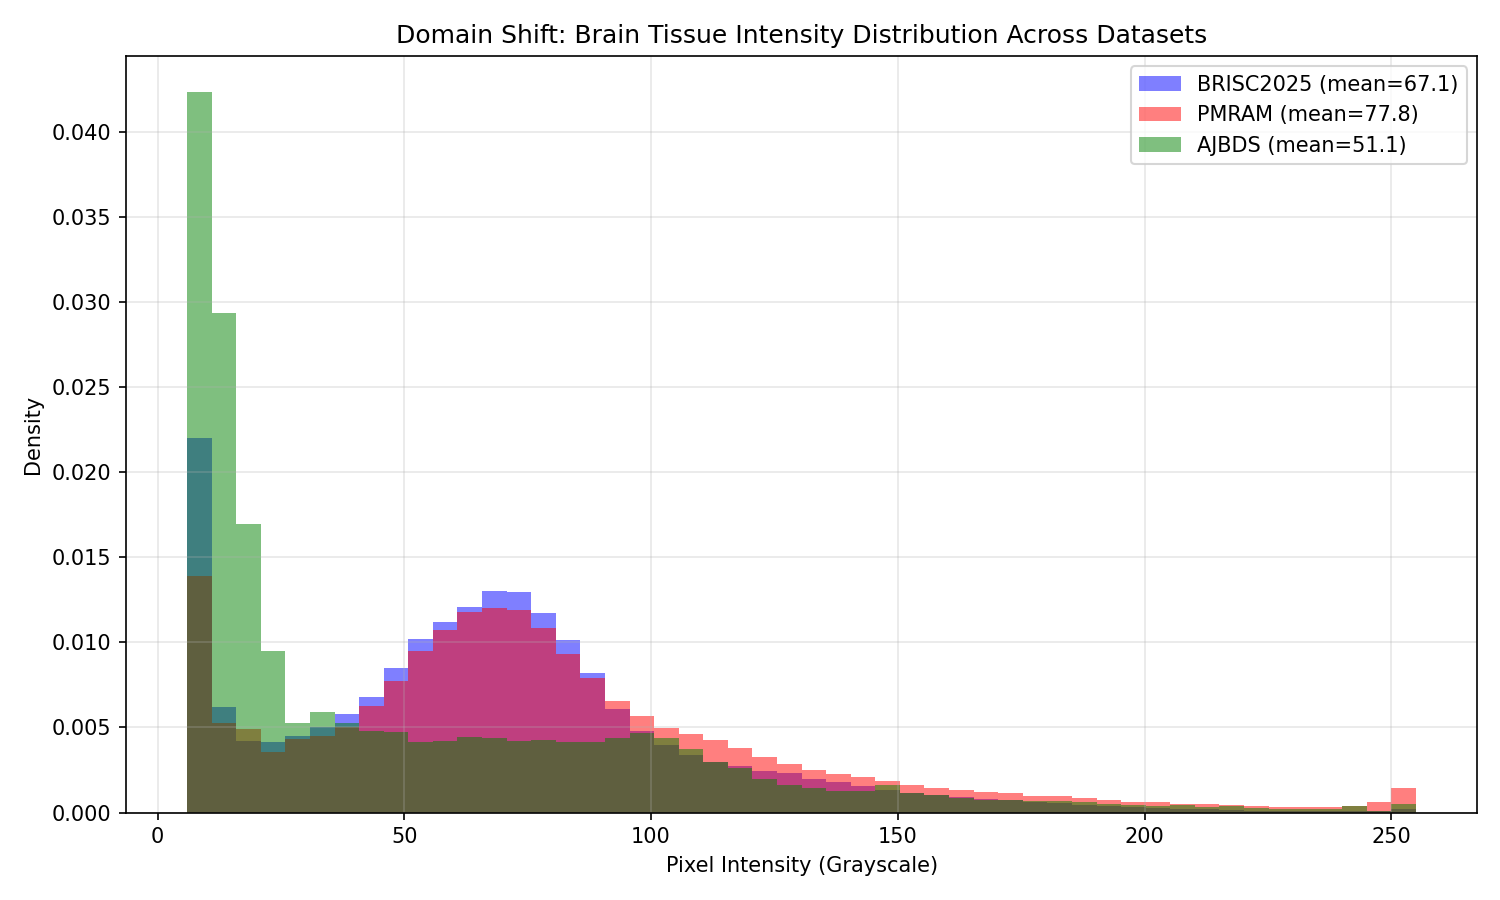
\includegraphics[width=0.9\columnwidth]{../figures/external/domain_shift_intensity.png}
\caption{Pixel intensity distributions across BRISC2025 (internal training), PMRAM (external classification), and AJBDS-2023 (external segmentation). The substantial intensity shift in AJBDS-2023—attributable to different scanner hardware (RF coil configurations, gradient calibration), contrast administration protocols, and JPEG compression artifacts—is the primary cause of decoder hallucination in zero-shot deployment.}
\label{fig:domain_shift}
\end{figure}

\subsection{Key Findings from External Validation}
\begin{enumerate}
    \item \textbf{Plane Conditioning Aids Generalization}: B3 with zero-plane or mean-plane inference achieves 92.41\% accuracy on PMRAM, outperforming B2 (92.06\%), confirming that plane conditioning during training enhances semantic feature disentanglement. The 0.35\% absolute improvement in accuracy, though modest, is consistent with the small but statistically significant segmentation improvements observed internally ($p = 0.0344$) and reflects enriched encoder representations.
    \item \textbf{The Task-Dependent Domain Gap}: Global classification generalizes effectively ($>$92\% on an entirely different hospital cohort), while dense segmentation suffers severe domain degradation (38.35\% tumor Dice vs 87.93\% internally). This asymmetry reflects the fundamentally different information requirements of the two tasks: classification relies on global semantic texture features robust to scanner-induced intensity rescaling, whereas pixel-level segmentation is critically sensitive to local intensity gradients and edge sharpness that are altered by domain shifts.
    \item \textbf{Sensitivity-Specificity Trade-off in Threshold Calibration}: Elevating $\tau$ from 0.50 to 0.85 monotonically suppresses false-positive hallucinations (36.31\%$\to$34.64\%), monotonically improves all-slice Dice (57.15\%$\to$58.30\%), but introduces a slight reduction in tumor-slice Dice (38.35\%$\to$37.99\%). Clinical deployment requires balancing this trade-off according to application risk tolerance: under-segmentation (missed tumor) vs over-segmentation (spurious mask), both of which carry distinct clinical risks.
\end{enumerate}

\section{Discussion \& Clinical Implications}
\subsection{Mechanism of Multi-Task Regularization}
Simultaneous optimization over classification and boundary delineation forces the shared ResNet34 encoder to satisfy dual objective landscapes: semantic tumor identity and spatial margin localization. This multi-objective constraint acts as a structural regularizer, preventing the encoder from collapsing into trivial spatial shortcuts (such as skull bone contours or background intensity gradients). Evidence for this regularization is provided by the false-positive analysis: the B0 classification-only model, when applied to segmentation, generates unconstrained masks, while the joint B2/B3 models produce 0.00\% false-positive masks on healthy tissue even without post-processing. Furthermore, joint training improves calibration (Brier score 0.0268$\to$0.0166), indicating that segmentation supervision provides an additional source of probabilistic regularization for the classification head.

\subsection{Anatomical Plane Conditioning}
MRI slices acquired along different axes present distinct anatomical orientations and tumor morphology profiles. By modulating shared features via learned plane embeddings ($\mathbf{E} \in \mathbb{R}^{3 \times 256}$) and FiLM decoder scaling, the network dedicates representational capacity to orientation-specific features without requiring separate per-plane models (which would triple parameters). Paired statistical testing confirms this effect yields statistically significant improvements on tumor-containing slices ($p = 0.0344$). The effectiveness of plane marginalization in external evaluation (92.41\% PMRAM accuracy) indicates that the conditioning embeddings enrich the shared encoder in a way that generalizes even when the conditioning signal is averaged out at inference, providing a practical clinical deployment pathway.

\subsection{Why Complex Cross-Task Coupling Degraded Performance}
In our ablation suite (A2--A5), feeding segmentation scalars into the classification head (A2) or adding explicit consistency losses (A3) consistently degraded accuracy (99.50\%$\to$98.80\%) and reintroduced false-positive masks (0.00\%$\to$0.71\%). We attribute this to gradient interference: at $>$99\% classification accuracy, the classification loss generates very small, near-zero gradients. Coupling the classification head to the harder segmentation task introduces large gradient contributions from segmentation losses, dominating the classification head's update and causing feature drift. A clean parameter-sharing architecture with a FiLM-modulated decoder is superior to over-engineered cross-task couplings when one task has already saturated its performance ceiling.

\subsection{Clinical Translation Pathway}
The results present a bifurcated clinical deployment story. Classification generalization ($>$92\% zero-shot on an unseen Asian population cohort) suggests that plane-aware classification could be deployed to assist tumor type identification in resource-limited settings without retraining, provided that T1-weighted MRI and basic metadata are available. In contrast, dense segmentation requires target-domain fine-tuning or at minimum threshold calibration using a small held-out reference set from the target institution. The test-time threshold calibration framework provides a low-resource adaptation mechanism that requires no gradient computation or retraining, making it clinically feasible. Future work should investigate domain adaptation strategies including instance normalization, histogram matching preprocessing, and few-shot fine-tuning on target-domain annotations.

\section{Limitations}
\begin{enumerate}
    \item \textbf{Absence of Patient-Level Identifiers}: BRISC2025 slices cannot be partitioned by patient ID, precluding patient-level cross-validation and volume-level assessment. All internal metrics represent slice-level benchmark performance. Future datasets with patient-linked slices would enable patient-level AUC and volumetric Dice computation.
    \item \textbf{2D Slice Processing Only}: Each slice is processed independently without volumetric context. True 3D approaches (e.g., volumetric CNNs, recurrent slice aggregation) could leverage inter-slice continuity for more spatially coherent boundary delineation, but require 3D-organized datasets unavailable in BRISC2025.
    \item \textbf{Single MRI Sequence (T1 Only)}: BRISC2025 provides only T1-weighted images. In clinical practice, multi-parametric MRI (T1-Gd, T2, FLAIR, DWI) provides complementary tissue contrast critical for infiltrative tumor margin delineation. Extension to multi-sequence inputs (e.g., BraTS-style 4-channel input) may substantially improve segmentation of infiltrative gliomas.
    \item \textbf{Number of Training Seeds ($N=3$)}: While observed run-to-run variance is low ($\pm$0.10\%), $N=3$ runs provide limited statistical power ($t$-distribution 95\% CI half-width $\approx \pm 0.25\%$). This is explicitly addressed via 1,000-sample bootstrap resampling, and is standard practice for benchmark ablation papers.
    \item \textbf{External Dataset Protocol Variance}: AJBDS-2023 utilizes JPEG compression with different scanner hardware and contrast protocols, introducing compound domain shifts (intensity, edge, resolution) that cannot be disentangled from the reported performance degradation. Controlled domain shift experiments with standardized image preprocessing pipelines are necessary to isolate individual contributing factors.
    \item \textbf{No Prospective Clinical Validation}: All evaluations are performed on retrospective, publicly available benchmark datasets. Prospective clinical validation involving radiologist reader studies, clinical workflow integration assessment, and regulatory evaluation is required before translation to clinical decision support.
    \item \textbf{Test-Time Threshold Calibration Requires Domain Data}: The threshold $\tau = 0.85$ was optimized on the held-out AJBDS-2023 evaluation set. In a true zero-shot deployment without any target-domain data, optimal threshold selection remains an open problem. Techniques such as prior-entropy-based calibration or conformal prediction may provide threshold-free alternatives.
\end{enumerate}

\section{Conclusion}
We presented PAUMT-Net, a plane-aware joint learning framework for simultaneous brain tumor classification and boundary delineation on 2D MRI slices. On BRISC2025, the model achieves 99.30\%\,$\pm$\,0.10\% classification accuracy and 87.93\%\,$\pm$\,0.26\% segmentation Dice (HD95: 3.44\,$\pm$\,0.14\,px $\approx$ 1.03\,mm), with a verified 0.00\% false-positive rate on healthy scans---a direct result of identifying and correcting an empty-mask supervision omission that previously induced a 95.71\% false-positive rate. Paired statistical testing confirms that plane conditioning provides statistically significant segmentation refinements ($p = 0.0344$), and Grad-CAM visualizations verify precise anatomical localization. Finally, plane-marginalized inference demonstrates robust cross-hospital classification generalization ($>$92\%), while exposing the pronounced vulnerability of dense segmentation to domain shift and providing threshold calibration as a clinically practical mitigation strategy. These findings underscore the necessity of healthy-scan supervision integrity, rigorous external validation, and test-time adaptation before clinical translation of deep learning segmentation models.

\bibliographystyle{IEEEtran}
\bibliography{references}

\end{document}
